\documentclass[12pt, a4paper, twoside, openright]{article}		% 5p gir 2 kolonner pr side. 1p gir 1 kolonne pr side.
%\journal{students}
\usepackage[T1]{fontenc} 						% Vise norske tegn.
% \usepackage[latin1]{inputenc}		% Velger tengsettet i dette dokumentet			
\usepackage[english]{babel}		
\usepackage[utf8]{inputenc}
\usepackage{graphicx}
\usepackage{hyperref}
\usepackage{amsmath,amssymb}
\usepackage{esint}
\usepackage[output-decimal-marker = {,}]{siunitx}
\usepackage[font=footnotesize,labelsep=period,labelfont=bf,margin=1cm]{caption}
\usepackage{import}
\usepackage{caption}
\usepackage{subcaption}
\usepackage[margin=2.5cm]{geometry}
\usepackage{lipsum}
\usepackage[numbers]{natbib}
\usepackage[nottoc,numbib]{tocbibind}
\usepackage{titlesec}
\usepackage{emptypage}
\let\oldsection\section
\def\section{\cleardoublepage\oldsection}
\newcommand{\sectionbreak}{\clearpage}
\usepackage{afterpage}
\newcommand\blankpage{%
    \null
    \thispagestyle{empty}%
    \addtocounter{page}{-1}%
    \newpage}


\setcounter{totalnumber}{5}
\renewcommand{\textfraction}{0.05}
\renewcommand{\topfraction}{0.95}
\renewcommand{\bottomfraction}{0.95}
\renewcommand{\floatpagefraction}{0.35}
\renewcommand{\d}[1]{\ensuremath{\operatorname{d}\!{#1}}}
\DeclareRobustCommand{\orderof}{\ensuremath{\mathcal{O}}}
\setlength\parindent{24pt}
\numberwithin{equation}{section}



\setcounter{totalnumber}{5}
\renewcommand{\textfraction}{0.05}
\renewcommand{\topfraction}{0.95}
\renewcommand{\bottomfraction}{0.95}
\renewcommand{\floatpagefraction}{0.35}

\makeatletter
\def\ps@pprintTitle{%
  \let\@oddhead\@empty
  \let\@evenhead\@empty
  \let\@oddfoot\@empty
  \let\@evenfoot\@oddfoot
}
\makeatother

\begin{document}

\begin{titlepage}

\newcommand{\HRule}{\rule{\linewidth}{0.5mm}} % Defines a new command for the horizontal lines, change thickness here

\center % Center everything on the page
 
%----------------------------------------------------------------------------------------
%	HEADING SECTIONS
%----------------------------------------------------------------------------------------

%\textsc{\LARGE Norwegian University of \\ \vspace{0.3cm} Science and Technology}\\[1.5cm] % Name of your university/college
\textsc{\Large Specialization project in theoretical physics}\\[0.5cm] % Major heading such as course name
%\textsc{\large Minor Heading}\\[0.5cm] % Minor heading such as course title

%----------------------------------------------------------------------------------------
%	TITLE SECTION
%----------------------------------------------------------------------------------------

\HRule \\[0.4cm]
{ \huge \bfseries Magnetization dynamics of domain walls and skyrmions in micromagnetics}\\[0.4cm] % Title of your document
\HRule \\[1.5cm]
 
%----------------------------------------------------------------------------------------
%	AUTHOR SECTION
%----------------------------------------------------------------------------------------

\begin{minipage}{0.4\textwidth}
\begin{flushleft} \large
\emph{Author:}\\
\O yvind \textsc{Johansen} % Your name
\end{flushleft}
\end{minipage}
~
\begin{minipage}{0.4\textwidth}
\begin{flushright} \large
\emph{Supervisor:} \\
Prof. Jacob \textsc{Linder} % Supervisor's Name
\end{flushright}
\end{minipage}\\[4cm]

% If you don't want a supervisor, uncomment the two lines below and remove the section above
%\Large \emph{Author:}\\
%John \textsc{Smith}\\[3cm] % Your name

%----------------------------------------------------------------------------------------
%	DATE SECTION
%----------------------------------------------------------------------------------------

{\large \today}\\[3cm] % Date, change the \today to a set date if you want to be precise

%----------------------------------------------------------------------------------------
%	LOGO SECTION
%----------------------------------------------------------------------------------------


\includegraphics[width=0.5\textwidth]{Figures/ntnu-logo.png} % Include a department/university logo - this will require the graphicx package
 
%----------------------------------------------------------------------------------------

\vfill % Fill the rest of the page with whitespace

\end{titlepage}

%\title{Magnetization dynamics of domain walls and skyrmions in micromagnetics}
%\author{\O yvind Johansen}
%\date{\today}

%\maketitle
\afterpage{\blankpage}
\pagenumbering{roman}

\section*{Summary}
In this project we study the origin of different magnetization patterns such as magnetic domain walls and magnetic skyrmions. These magnetic structures are found by minimizing the micromagnetic energy, where the exchange energy, anisotropic energy and demagnetization energy are considered. In the case of magnetic skyrmions the energy contribution from the Dzyaloshinskii--Moriya interaction is also taken into account. The extended Landau--Lifshitz--Gilbert equation is then presented and used to describe the motion of the magnetization patterns when a spin-polarized current or an external magnetic field is applied. For the motion of the magnetic domain walls it is found that the relation between the translational speed of the domain wall and the strength of the applied current or magnetic field is linear up to some critical value. If the currents or fields are stronger than the critical value it is shown that a Walker breakdown occurs. For the motion of skyrmions it is shown that the velocity of the skyrmion is linearly related to the strength of the applied current for small currents. There are found to be two velocity components; one parallel to the direction of the motion of the conduction electrons, and a velocity component perpendicular to the direction of the applied current which originates from the skyrmion Hall effect. The translational speed of the skyrmion is also found to be dependent on the skyrmion profile. In the case of an applied magnetic field it is discovered that the skyrmion rotates and changes its profile compared to the equilibirum profile in the absence of a magnetic field.
\newpage

\section*{Preface}
This thesis is the end result of a specialization project in quantum condensed matter theory and is part of a five year integrated Master's programme at the Norwegian University of Science and Technology. Its purpose is to gain knowledge and insight in a special field in physics as a preparation for the master thesis.

I would like to thank my supervisor Jacob Linder for providing helpful information and valuable input throughout this project.\\

\begin{minipage}{0.95\textwidth}
\begin{flushright}
\O yvind Johansen \\
Trondheim, Norway \\
November 2015
\end{flushright}
\end{minipage}\\[4cm]

\newpage

\tableofcontents

\newpage
\afterpage{\blankpage}

\pagenumbering{arabic}

\section{Introduction}
Electronics has for a long time been the most commonly used science in information technology. In the recent decades, however, a contender has emerged in spintronics, where the intrinsic spin of the electron is utilized instead of its electric charge. Spintronics is closely related to magnetic materials, a good example of which is shown by an experiment performed by Johnson and Silsbee in 1985 \cite{JohnsonSilsbee1985}, where an electric current passing through a ferromagnet was seen to have the same spin-polarization as the magnetic material. The spins in an electric current therefore interact with the magnetic moments in a magnet.

Magnetic materials have been studied closely over the last century. Magnets are today known to be divided into smaller regions of a uniform magnetization, known as magnetic domains. These magnetic domains are separated by solitons called domain walls. These solitons have different structures, one of which was shown by Bloch in 1932 \cite{Bloch1932}. 

The magnetic solitons occur as to minimize the energy in the magnetic material, and is therefore an equilibrium effect. As magnetic moments interact with magnetic fields, the solitons can move away from equilibrium and gain dynamical properties. The time evolution of these solitons was first described by an equation of motion proposed by Landau and Lifshitz in 1935 \cite{LandauLifshitz1935}, which was based on a damped precession around an effective magnetic field that included internal and external effects. The damping term in the equation proposed by Landau and Lifshitz was then replaced by Gilbert in 1955 \cite{Gilbert2004Classics} to include the time derivative, which agreed better with experiments. This equation was then extended by Slonczewski in 1996 to include the interaction between the spins in an electric current and the local magnetization in the magnet \cite{Slonczewski1996}.

The magnetic solitons can be used for information storage in form of bits. An example of this that is widely used in hard drives and magnetoresistive random-access-memory today is the giant magnetoresistance (GMR) effect discovered independently by Fert and Gr\"{u}nberg in 1988 \cite{Fert1988} \cite{Grunberg1989}, which they won the Nobel prize in physics for in 2007. This effect occurs in a system with three different layers; a fixed magnetic layer, a non-magnetic layer, and a magnetic layer with reversable magnetization. If the last magnetic layer has the same magnetization direction as the fixed layer, there is a low resistance to an electrical current passing through the system. If the last layer has the opposite magnetization direction of the fixed layer, however, the resistance increases significantly. This is therefore suitable to describe a bit, which has two possible values. The magnetization direction in the last layer can be manipulated by either applying a spin-polarized current, or an external magnetic field. This corresponds to moving the magnetic domain wall separating the two different magnetic domains (parallel and anti-parallel to the fixed layer), and can be used to write and rewrite information. In this project we will study the dynamical properties of this magnetic soliton as a function of current and external magnetic field.

In the last decade, another type of magnetic soliton known as a magnetic skyrmion has been of a considerable interest as a new possibility as an information carrier in spintronics. The name skyrmion stems from the phycicist Tony Skyrme, who described baryons and mesons as topological solitons in 1962 \cite{Skyrme1962}. The magnetic skyrmion is a two-dimensional topologically-protected object found in chiral magnets, and has a vortex-like structure. The magnetic skyrmion was observed experimentally in 2009 \cite{Muhlbauer2009}. As the magnetic skyrmion is topologically protected, it is a stable magnetization configuration and behaves as a quasiparticle. 

The interest in magnetic skyrmion as information carriers was increased when it was shown that these "quasiparticles" can be manipulated by a current density of several orders magnitude less than that which was required to manipulate magnetic domain walls \cite{Jonietz2010}. In this project the profile of the magnetic skyrmion is studied, as well as its dynamical properties when a spin-polarized current is applied. To set the stage for this, we first study the more well known magnetic domain walls. This way any difference in the dynamical properties between the domain walls and skyrmions become more clear: we can see if the phenomena that occur in domain wall motion also apply for skyrmions, or if we have any new phenomena in the skyrmion case.

\section{Energy terms in micromagnetics}\label{sec:MicromagneticEnergy}
\subsection{Anisotropic energy}
Magnetic materials may be anisotropic, meaning that certain directions of the magnetization in the material are more energetically favorable than others. This stands in contrast to isotropic materials where the energy is independent of the direction of the magnetization, assuming uniform magnetization. There are several possible causes for anisotropy in a material, the most common one being the crystalline structure in the material. One of the most important causes of magnetocrystalline anisotropy is the spin-orbit coupling interaction. This interaction arises from the fact that in the restframe of the electron, the proton is orbiting the electron, thereby creating a varying electric field. Since the electric field is varying, Maxwell's equations say that there will also be a corresponding magnetic field. This magnetic field is proportional to the angular momentum $\vec{L}$ of the electron. The electron also has a magnetic moment $\vec{\mu}$, proportional to its spin $\vec{S}$, that will interact with the magnetic field. The energy is lowest when the magnetic moment and field are aligned, which we will see when discussing the Zeeman energy later. Combining the spin--orbit interaction with the orientation of the atoms in the lattice it is possible that some directions in the material are easier magnetized than others. This is magnetocrystalline anisotropy. The shape of the magnetic particles may also cause anistropy in the material, which will be briefly discussed in the section on the demagnetization energy. 

In anisotropic magnetic materials one defines different axes; the easy, intermediate and hard axes. If the magnetization is oriented along the easy axis, the anisotropic energy is at its minimum value. Similarly, if the magnetization is oriented along the hard axis the anisotropic energy is at its maximum value. The intermediate axis is the direction along which there is a saddlepoint in the anisotropic energy. In most materials the anisotropic energy is the same for both possible orientations of the magnetization along the axes. When this is the case, the terms in the anisotropic energy can only contain even powers of the components in the magnetization vector.

\subsubsection{Uniaxial anisotropy}
The simplest form of anisotropy is the case where there is only one axis that the anisotropic energy varies with. This is known as uniaxial anisotropy. This can often be found in crystal structures with a single principal axis, such as the hexagonal and simple tetragonal lattices. The uniaxial anisotropic energy is determined by the component of the unit vector of the magnetization that points parallel to the axis in the material that is the easiest (or hardest) direction to magnetize the material. If we consider a uniform magnetization $\vec{M} = \left[M_x, M_y, M_z\right]$ and let one of the two directions along the axis in the material that defines an extremal value in the anisotropic energy be the unit vector $\hat{n}$ (for example, if we have a uniaxial anisotropy along the $z$-axis, $\hat{n}$ can be $\pm\hat{z}$), the anisotropic energy must be on the form
\begin{align}
\label{eq:uniaxialanisotropy}
E_A = V \sum_{i=0}^{\infty} K_i \left(\frac{\vec{M}\cdot\hat{n}}{M_s}\right)^{2i}
\end{align}
if there is to be no preferential direction with respect to energy along the axis. This can be seen as we restrict ourselves to even powers, so both of the possible choices $\hat{n}=\pm\hat{z}$ lead to the same anisotropic energy $E_A$ in the case of a uniaxial anisotropy along the $z$-axis. In the equation above $V$ is the volume, $M_s = |\vec{M}|$ the saturation magnetization and $K_i$ are the anisotropy constants. By only considering the lowest order in the anisotropic energy it becomes
\begin{align}
\label{eq:uniaxialanisotropy_v2}
E_A = K V \left(\frac{\vec{M}\cdot\hat{n}}{M_s}\right)^2
\end{align}
by ignoring the constant energy term as that only leads to a constant shift in the energy. If $K < 0$ the axis that $\hat{n}$ points along is then the easy axis as the system is in a lower energy state when the magnetization points along $\pm\hat{n}$, and if $K > 0$ the axis is the hard axis as the system is then in a higher energy state when the magnetization points along $\pm\hat{n}$. Note that if we have a non-uniform magnetization we let

\begin{align*}
\vec{M} &\rightarrow \vec{M}(\vec{r}), \\
V &\rightarrow \int \d V.
\end{align*}

\subsubsection{Cubic anisotropy}
Many magnetic materials, such as iron, have cubic crystal structures. This can give rise to cubic anisotropy in the magnetic material. To describe cubic anisotropy it can be useful to introduce directional cosines that give the component of a unitary vector along the $x$-, $y$- and $z$-axes. Using spherical coordinates, these directional cosines are defined to be $\alpha = \sin\theta\cos\phi$, $\beta = \sin\theta\sin\phi$, $\gamma = \cos\theta$. Note that the directional cosines can also be written in terms of the magnetization, so that $\alpha = M_x/M_s$, $\beta = M_y/M_s$ and $\gamma = M_z/M_s$. If there is to be no preferential direction with respect to energy along the crystal axes, the anisotropic energy can only contain even powers of $\alpha$, $\beta$ and $\gamma$. In addition, to have cubic symmetry in the anisotropic energy, the energy must be invariant under any interchanges among the directional cosines \cite{Kittel:ISSP}. The first term in the anisotropic energy that depends on the directional cosines will therefore be proportional to $\alpha^2+\beta^2+\gamma^2$, but using the definitions of the directional cosines we find that
\begin{align}
\label{eq:cosinesconstraint}
\alpha^2+\beta^2+\gamma^2 = \frac{M_x^2+M_y^2+M_z^2}{M_s^2} = \frac{|\vec{M}|^2}{|\vec{M}|^2} = 1.
\end{align}
This term is therefore just a constant, so to find a term that varies with the directional cosines we must go to fourth order:
\begin{align}
\label{eq:cubicanisotropy}
E_A = E_A^{(0)} + \int (K_1 (\alpha^2\beta^2+\alpha^2\gamma^2+\beta^2\gamma^2) + \ldots ) \d V.
\end{align}
The sixth order term would be on the form $K_2 V \alpha^2\beta^2\gamma^2$ and so on. If one looks at the form of the energy in \eqref{eq:cubicanisotropy} one can determine the easy and hard axes in the material. The integrand has to be minimized along the easy axes, and maximized along the hard axes. If one only considers the fourth order terms in the energy, we have to minimize and maximize the function $K_1 (\alpha^2\beta^2+\alpha^2\gamma^2+\beta^2\gamma^2)$ with the constraint given by \eqref{eq:cosinesconstraint}. Using Lagrange multipliers, this breaks down to solving 
\begin{align}
\nabla f(\alpha, \beta, \gamma) &= \lambda \nabla g(\alpha, \beta, \gamma), \\
g(\alpha, \beta, \gamma) &= 0,
\end{align}
with
\begin{align}
f(\alpha, \beta, \gamma) &= K_1 (\alpha^2\beta^2+\alpha^2\gamma^2+\beta^2\gamma^2), \\
g(\alpha, \beta, \gamma) &= \alpha^2+\beta^2+\gamma^2 - 1,\\
\nabla &= \left[\frac{\partial}{\partial\alpha}, \frac{\partial}{\partial\beta}, \frac{\partial}{\partial\gamma}\right].
\end{align}
This gives us the following set of equations to solve:
\begin{align*}
2K_1\alpha (\beta^2+\gamma^2) &= 2\alpha\lambda, \\ 
2K_1\beta (\alpha^2+\gamma^2) &= 2\beta\lambda, \\ 
2K_1\gamma (\alpha^2+\beta^2) &= 2\gamma\lambda, \\ 
\alpha^2+\beta^2+\gamma^2 - 1 &= 0.
\end{align*}
One can easily see that one solution of the equations is given by $\lambda = 0$, one of the directional cosines being $\pm 1$ and the other two being 0. Inserting this solution into $f(\alpha, \beta, \gamma)$ we get $f = 0$.

Assuming only one of the directional cosines is 0, for example $\gamma$, one gets
\begin{align*}
K_1 \beta^2 &= \lambda, \\ 
K_1 \alpha^2 &= \lambda.
\end{align*}
Using the constraint in \eqref{eq:cosinesconstraint} one finds $\lambda = K_1/4$, and both non-zero directional cosines being $\pm 1/2$. Inserting this solution into $f(\alpha, \beta, \gamma)$ we get $f = K_1/4$.

Assuming none of the directional cosines are 0, one gets
\begin{align*}
K_1 (\beta^2+\gamma^2) &= \lambda, \\ 
K_1 (\alpha^2+\gamma^2) &= \lambda, \\ 
K_1 (\alpha^2+\beta^2) &= \lambda.
\end{align*}
Using the constraint in \eqref{eq:cosinesconstraint} one finds $\lambda = 2K_1/3$, and each of the directional cosines being $\pm 1/\sqrt{3}$. Inserting this solution into $f(\alpha, \beta, \gamma)$ we get $f = K_1/3$. This means that if $K_1 > 0$ the energy is minimized by the first solution, making the $x$-, $y$- and $z$-axes the easy axes. The hard axes are then given by the third solution which corresponds to the four axes $x = \pm y = \pm z$, $x = \pm y = \mp z$. If $K_1 < 0$ the energy is maximized by the first solution and minimized by the third, so that the easy and hard axes switch from the case when $K_1 > 0$. The second solution denotes a local minimum if $K_1<0$ and a local maximum if $K_1>0$. The second solution does not give any intermediate axes, as there is no saddle point in the energy.


\subsection{Demagnetization energy}
The magnetic dipoles inside a ferromagnet will generate a magnetic field, known as the demagnetizing field. This name stems from the behavior of the field, as it will try to reduce the total magnetic moment in the magnet. This is because a high magnetic moment in the magnet will generate a strong external magnetic field, which costs energy. Magnetic materials consist of magnetic dipoles, if the magnetization is uniform there will be no poles inside the magnet, as the positive and negative poles cancel each other out. There will, however, be a positive pole at one surface of the magnet and a negative pole at the opposing surface that do not cancel out. This causes a large total magnetic moment in the magnet, as it is proportional to the length between the poles. To minimize the total magnetic moment and thereby the energy, the demagnetizing field will therefore create magnetic domains, where the different domains have uniform magnetization in different directions. There is a limit to how small the domains can be, as the exchange interaction will begin to dominate on short ranges, which we will discuss later. 

The energy in a ferromagnet will depend on the orientation of the magnetic dipoles with respect to the demagnetizing field created by the other magnetic dipoles. This demagnetization energy is given by

\begin{align}
\label{eq:demagenergy}
E_D = -\frac{\mu_0}{2}\int \d {^3}r \vec{M}(\vec{r})\cdot\vec{H}_D(\vec{r}),
\end{align}
with $\vec{H}_D$ being the demagnetization field. From this equation it looks like the demagnetizing field will attempt to align the magnetization with itself, which is not the behavior that was discussed earlier. One can not make this conclusion yet, however, as the demagnetizing field is at this point an unknown function of the magnetization $\vec{M}$. To determine the demagnetization energy one needs to find the magnetic field generated by a magnetic dipole $\vec{M}$. The magnetic induction $\vec{B}(\vec{r})$ is defined as
\begin{align}
\vec{B}(\vec{r}) = \nabla \times \vec{A}(\vec{r}),
\end{align}
with the vector potential $\vec{A}(\vec{r})$ of a magnetic dipole being known as
\begin{align}
\vec{A}(\vec{r}) = \frac{\mu_0}{4\pi}\frac{\vec{M}\times\vec{r}}{r^3}.
\end{align} 
Using the Einstein summation convention and the Levi--Civita tensor $\varepsilon_{ijk}$ one can then find the magnetic induction generated by a single magnetic dipole:
\begin{align*}
B_i &= \varepsilon_{ijk} \partial_j A_k \\
&= \varepsilon_{kij}\varepsilon_{klm} \frac{\mu_0}{4\pi}\partial_j\frac{M_l r_m}{r^3} \\
&= (\delta_{il}\delta_{jm}-\delta_{im}\delta_{jl})\frac{\mu_0}{4\pi}\left(\frac{M_l\delta_{jm}}{r^3}-\frac{3M_lr_mr_j}{r^5}\right) \\
&= \frac{\mu_0}{4\pi}\left(\frac{3(\vec{M}\cdot\vec{r})r_i}{r^5}-\frac{M_i}{r^3}\right).
\end{align*}
This means that the magnetic field strength of the demagnetization field generated by the entire magnet at a position $\vec{r}$ is
\begin{align}
\label{eq:demagfield}
\vec{H}_D = \frac{1}{4\pi} \int \d {^3}r' (\frac{3(\vec{M}(\vec{r'}) \cdot (\vec{r}-\vec{r'})) (\vec{r}-\vec{r'})}{|\vec{r}-\vec{r'}|^5}-\frac{\vec{M} (\vec{r'})}{|\vec{r}-\vec{r'}|^3}).
\end{align}
\begin{figure}[h!]
\begin{center}
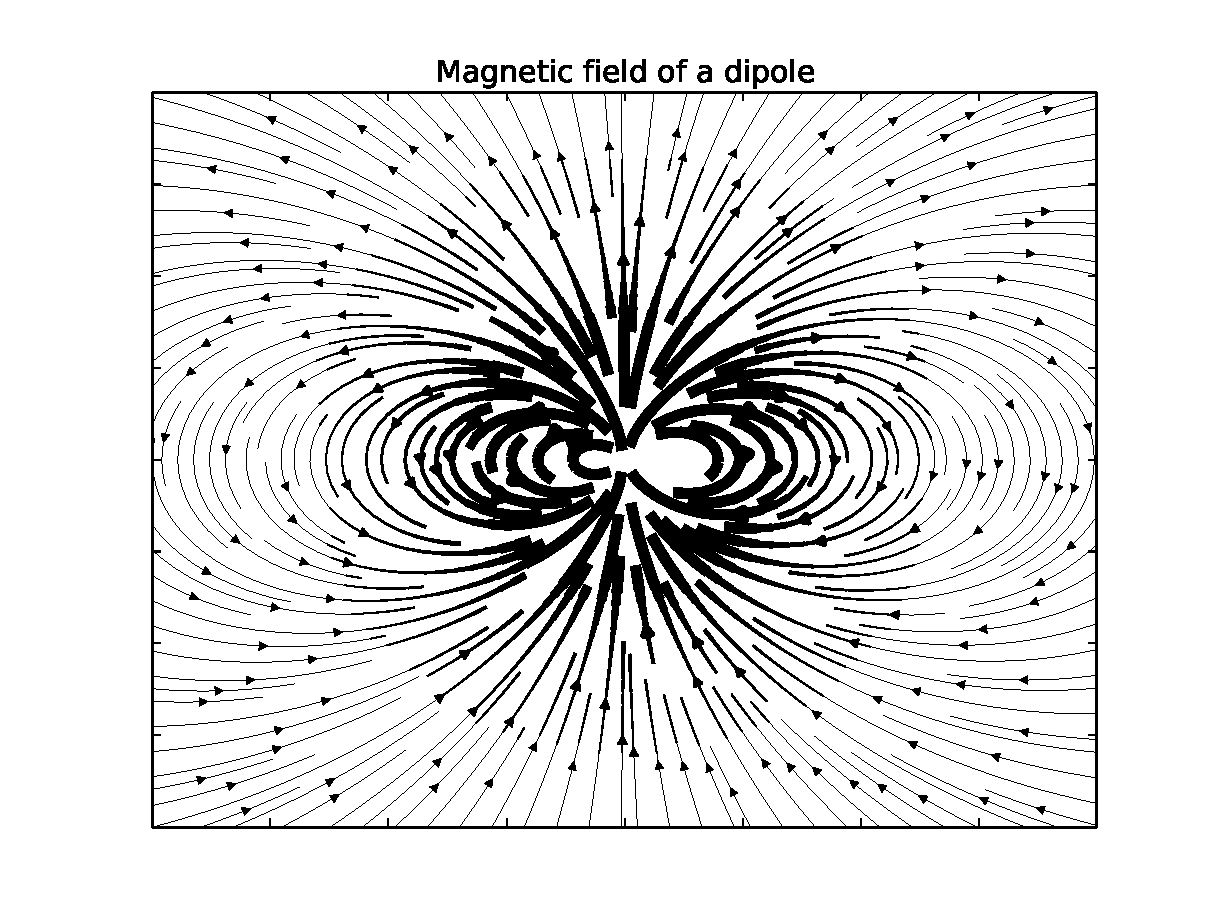
\includegraphics[width=0.8\textwidth]{Figures/dipole_field.pdf} 
\caption{The magnetic field generated by a single magnetic dipole located at the origin pointing in the $y$-direction. Broad field lines indicate a strong magnetic field.}
\label{fig:dipole_field} 
\end{center}
\end{figure}
In Figure \ref{fig:dipole_field} one can see that the demagnetizing field has a tendency to point in a different direction than the magnetization. At a position that is perpendicular to the magnetization the field is completely anti-aligned with the magnetization. Inserting \eqref{eq:demagfield} into \eqref{eq:demagenergy} one finds that the energy is
\begin{align}
\label{eq:demagenergy_mag}
E_D = \frac{\mu_0}{8\pi} \int \d {^3}r \int \d {^3}r' (\frac{\vec{M} (\vec{r}) \cdot \vec{M} (\vec{r'})}{|\vec{r}-\vec{r'}|^3} - \frac{3(\vec{M}(\vec{r}) \cdot (\vec{r}-\vec{r'})) (\vec{M}(\vec{r'}) \cdot(\vec{r}-\vec{r'}))}{|\vec{r}-\vec{r'}|^5}).
\end{align}
The energy is at its minimum when the total magnetization in the magnet goes to zero, the demagnetizing field will therefore try to reduce the total magnetic moment in the magnet as discussed earlier. 
The integrand in \eqref{eq:demagenergy_mag} can be rewritten in a tensor form \cite{kruger2006current}. Using the relation
\begin{align}
\partial_i \frac{1}{|\vec{r}-\vec{r'}|} = -\frac{r_i-r_i'}{|\vec{r}-\vec{r'}|^3}
\end{align}
it can be verified that
\begin{align*}
\partial_i\partial_j \frac{1}{|\vec{r}-\vec{r'}|} &= \partial_i\left(-\frac{r_j-r_j'}{|\vec{r}-\vec{r'}|^3}\right) \\
&= -\frac{\delta_{ij}}{|\vec{r}-\vec{r'}|^3}+3\frac{(r_i-r_i')(r_j-r_j')}{|\vec{r}-\vec{r'}|^5}.
\end{align*}
Defining the continuous demagnetization tensor to be
\begin{align}
N_{ij}(\vec{r}-\vec{r'}) = -\frac{1}{4\pi}\partial_i\partial_j \frac{1}{|\vec{r}-\vec{r'}|},
\end{align}
the demagnetization energy and field can then be written as
\begin{align}
E_D &= \frac{\mu_0}{2} \int \d {^3}r \int \d {^3}r' \vec{M}(\vec{r}) N(\vec{r}-\vec{r'})\vec{M}(\vec{r'}), \\
\vec{H}_D(\vec{r}) &= - \int \d {^3}r' N(\vec{r}-\vec{r'})\vec{M}(\vec{r'}).
\end{align}
Something worth noting is that if the demagnetization tensor $\bar{N}(\vec{r}-\vec{r'})$ is strictly diagonal, the energy can be written as
\begin{align}
E_D = \mu_0(N_{xx}M_x^2+N_{yy}M_y^2+N_{zz}M_z^2).
\end{align}
This is the case for ellipsoidal bodies \cite{kruger2006current}. This form of the demagnetization energy is similar to that of the uniaxial anisotropic energy in \eqref{eq:uniaxialanisotropy_v2}. This means that ellipsoidal magnetic particles cause shape anisotropy, assuming the magnetic particle is not spherical ($N_{xx} = N_{yy} = N_{zz}$).


\subsection{Zeeman energy}
The Zeeman energy describes the energy from the interaction between the magnetization of the magnet and an external field $\vec{H}_{Z}$. The Zeeman energy is on the same form as the demagnetization energy in \eqref{eq:demagenergy}, with the internally generated demagnetization field replaced by the external magnetic field:

\begin{align}
\label{eq:zeemanenergy}
E_Z = -\mu_0\int \d {^3}r \vec{M}(\vec{r})\cdot\vec{H}_{Z}(\vec{r}).
\end{align}
The factor 1/2 in the demagnetization energy is to account for double counting of the dipole interactions, and is therefore not included in the Zeeman energy as the magnetic moments only interact with an external field. The Zeeman energy is at its minimum when the magnetization is aligned with the external field.

\subsection{Symmetric exchange energy}
Spins on a lattice will have an exchange energy with their nearest neighbors, as given by the Heisenberg Hamiltonian
\begin{align}
\label{eq:heisenberg}
H = -J\sum_{<i, j>} \vec{S}_i\cdot\vec{S}_j = -\frac{J S^2}{M_s^2}\sum_{<i, j>} \vec{M}_i\cdot\vec{M}_j,
\end{align}
with $J$ being the exchange integral and $\vec{S}_{i,j}$ the dimensionless spins. This interaction between the spins is symmetric due to the properties of the dot product. For a ferromagnet the lowest exchange energy is when the spins are aligned, meaning $J>0$. In the Hamiltonian we sum over each nearest neighbor pair $<i, j>$. To perform the sum we look at the magnetization in the continuum limit, with a slowly varying magnetization. It is then possible to do a Taylor expansion around the magnetization $\vec{M}_i$. If one only looks at a Taylor expansion in the $x$-direction, it can be written as
\begin{align}
\label{eq:taylormag}
\vec{M}_{i+1} \approx \vec{M}_i + a\frac{\partial \vec{M}_i}{\partial x} + \frac{a^2}{2}\frac{\partial^2 \vec{M}_i}{\partial^2 x},
\end{align}
with $a$ being the lattice constant and $\vec{M}_{i+1}$ the magnetization at the neighboring site to $\vec{M}_i$ along the $x$-axis. Similar expansions can be done in the $y$- and $z$-directions. Using this we can take a look at the contribution to the energy from $\vec{M}_i$ and its nearest neighbors in \eqref{eq:heisenberg}. For simplicity we consider a cubic lattice with a lattice constant $a$. Each lattice site has six nearest neighbors in three dimensions. Applying \eqref{eq:taylormag} to find the contributions to the energy from the nearest neighbors in the $x$-direction located at $\pm a \hat{x}$ relative to $\vec{M}_i$, we find
\begin{align*}
\vec{M}_i\cdot\vec{M}_{i-1}+\vec{M}_i\cdot\vec{M}_{i+1} &= 2\vec{M}_i\cdot\vec{M}_i + (a - a) \vec{M}_i\cdot\frac{\partial \vec{M_i}}{\partial x} + a^2\vec{M}_i\cdot\frac{\partial^2 \vec{M}_i}{\partial^2 x} \\
&= 2M_s^2 + a^2\vec{M}_i\cdot\frac{\partial^2 \vec{M}_i}{\partial^2 x}.
\end{align*}
Doing the same calculation for the nearest neighbors in the $y$- and $z$-directions we get that the exchange energy density from the magnetization at one site and its nearest neighbors is
\begin{align}
\epsilon_i = -\frac{JS^2}{a^3}\left(6+\frac{a^2}{M_s^2}\vec{M}_i\nabla^2\vec{M}_i\right).
\end{align}
To find the total exchange energy in the magnet we integrate the energy density over the volume of the magnet, so that
\begin{align}
\label{eq:exchangeenergylaplace}
E_E = -\int \d {^3}r \frac{JS^2}{2aM_s^2} \vec{M}(\vec{r})\nabla^2\vec{M}(\vec{r}).
\end{align}
The constant term in the energy has been ignored, and the factor $1/2$ has been introduced to account for the double counting of the interaction pairs. The energy in \eqref{eq:exchangeenergylaplace} can be rewritten to a more common form. Introducing the index notation and using the Einstein summation convention, we integrate \eqref{eq:exchangeenergylaplace} by parts: 
\begin{align}
\label{eq:exchangeenergyDiv2}
\int \d {^3}r \vec{M}(\vec{r})\cdot\partial_i \partial_i \vec{M}(\vec{r}) = \int \d S \vec{M}(\vec{r})\cdot \frac{\partial}{\partial \hat{n}}\vec{M}(\vec{r}) - \int \d {^3}r \partial_i  \vec{M}(\vec{r})\cdot\partial_i \vec{M}(\vec{r}).
\end{align}
As $\vec{M}(\vec{r})$ is a vector of constant length, any change $\delta \vec{M}(\vec{r})$ must be perpendicular to $\vec{M}(\vec{r})$. This means that $\vec{M}(\vec{r})\cdot \frac{\partial}{\partial \hat{n}}\vec{M}(\vec{r}) = 0$, and the first term on the right hand side vanishes. The energy in \eqref{eq:exchangeenergylaplace} then becomes
\begin{align}
\label{eq:exchangeenergy}
E_E = \int \d {^3}r \frac{A}{M_s^2} \left((\frac{\partial}{\partial x}\vec{M}(\vec{r}))^2+(\frac{\partial}{\partial y}\vec{M}(\vec{r}))^2+(\frac{\partial}{\partial z}\vec{M}(\vec{r}))^2\right),
\end{align}
where we have introduced the exchange stiffness $A$. As one can see the energy depends on the variation in the magnetization in all directions, and is independent of which direction the magnetization changes, it is only dependent on the magnitude by which it changes. Because the exchange stiffness $A$ is positive in a ferromagnet, the exchange energy is higher the more the magnetization varies. To minimize the exchange energy the magnetization therefore has to vary slowly. On short ranges this effect is much stronger than the demagnetization and magnetocrystalline anisotropy. This is why neighbouring spins have a tendency to align in a ferromagnet, while on longer ranges when the demagnetization effect becomes stronger than the exchange interaction the spins tend to be anti-aligned.

\subsection{Antisymmetric exchange energy}
Certain magnetic materials also exhibit an antisymmetric exchange interaction between the spins in addition to the symmetric interaction. This is also known as the Dzyaloshinskii--Moriya interaction (DMI), and is given by the Hamiltonian
\begin{align}
\label{eq:DMI_Hamiltonian_S}
H_{DM} = \sum_{\langle i,j \rangle} \vec{D}_{ij} \cdot (\vec{S}_i\times\vec{S}_j),
\end{align}
where $\vec{D}_{ij}$ is a vector that depends on the symmetry of the material. This interaction favors a canting of the spins, unlike the symmetric exchange interaction where the favorable configurations were either parallel or antiparallel neighboring spins. It was first proposed by Dzyaloshinskii as a phenemenological reasoning \cite{Dzyaloshinskii1958}, and then Moriya later related this interaction to the spin-orbit coupling interaction \cite{Moriya1960}. If we absorb some constants into the magnitude of $\vec{D}_{ij}$, the Hamiltonian can also be written as
\begin{align}
\label{eq:DMI_Hamiltonian_M}
H_{DM} = \frac{1}{M_s^2}\sum_{\langle i,j \rangle} \vec{D}_{ij} \cdot (\vec{M}_i\times\vec{M}_j),
\end{align}
as the magnetization is proportional to the spin. To get a continuum form of the interaction energy in the micromagnetic limit, we follow the same procedure as for the symmetric exchange energy by performing a Taylor expansion in the different directions. Expanding in the $x$-direction we get
\begin{align}
\vec{M}_{i+1} \approx \vec{M}_i + a\frac{\partial \vec{M}_i}{\partial x},
\end{align}
with $a$ again being the lattice constant. As the form of the Hamiltonian is antisymmetric because of the properties of the cross product, we only look at the interaction pairs in one direction along a given axis. In cartesian coordinates the energy density then becomes
\begin{align}
\epsilon_{DM} = \frac{1}{M_s^2}\sum_i\vec{D}_{x_i}a_i\cdot(\vec{M}\times\frac{\partial \vec{M}}{\partial x_i}).
\end{align}
$\vec{D}_{x_i}$ is here a vector defined by the symmetry of the problem for the interaction pair in the $x_i$ direction ($x_i = x, y, z$). We will now consider different symmetries to see how this affects the antisymmetric interaction. Following the results provided by Moriya in \cite{Moriya1960}, we see that $\vec{D} = 0$ if there is a center of inversion symmetry. For the antisymmetric exchange interaction to be present, it is therefore necessary for the inversion symmetry to be broken. If there is an $n$-fold axis (where $n\geq2$) along the axis between the interaction pair, $\vec{D}$ will be parallel to that axis. If we then consider such a case where $\vec{D}_{x_i} = -\frac{D}{a_i} \hat{x}_i$, we find that
\begin{align}
\nonumber \epsilon_{DM} &= -\frac{D}{M_s^2} \left[ \hat{x}\cdot(\vec{M}\times\frac{\partial\vec{M}}{\partial x}) + \hat{y}\cdot(\vec{M}\times\frac{\partial\vec{M}}{\partial y}) + \hat{z}\cdot (\vec{M}\times\frac{\partial\vec{M}}{\partial z})\right] \\
\nonumber &= \frac{D}{M_s^2}\left[M_x(\frac{\partial M_z}{\partial y} - \frac{\partial M_y}{\partial z}) + M_y(\frac{\partial M_x}{\partial z} - \frac{\partial M_z}{\partial x}) + M_z(\frac{\partial M_x}{\partial y} - \frac{\partial M_y}{\partial x})\right] \\
&= \frac{D}{M_s^2} \vec{M}\cdot(\nabla\times\vec{M}). \label{eq:BulkDMI}
\end{align}
This is also known as the bulk form of the DMI energy density as we were considering a similar DMI in all spatial directions.

Let us now consider a case where the antisymmetric exchange interaction between two particles of the same type is transferred by a third particle of a different type. This can for example happen at an interface between two materials. According to Moriya the direction of $\vec{D}$ will then be parallel to the trigonal axis. If we consider an interface with a surface normal along the $z$ direction, the vectors $\vec{D}_{x_i}$ become
\begin{align}
\vec{D}_x = \frac{D}{a_x} \hat{y}, \hspace{10mm}
\vec{D}_y = - \frac{D}{a_y} \hat{x}, \hspace{10mm}
\vec{D}_z = 0,
\end{align}
where $D$ can be both positive and negative. This gives us the energy density
\begin{align}
\label{eq:InterfaceDMIe}
\epsilon_{DM} &= \frac{D}{M_s^2}\left[ \hat{y} \cdot(\vec{M}\times\frac{\partial\vec{M}}{\partial x}) - \hat{x} \cdot(\vec{M}\times\frac{\partial\vec{M}}{\partial y})\right] \\
&= \frac{D}{M_s^2}\left[ M_z (\nabla\cdot\vec{M}) - (\vec{M}\cdot\nabla)M_z\right]. \label{eq:IntDMI}
\end{align}
This is also known as the interface form of the DMI energy density.

As the DMI only occurs in select magnetic materials, we will not consider this contribution to the energy unless stated otherwise. It turns out, however, that this interaction is an important contribution to the form of magnetic skyrmions. This is because it allows a lowering of the energy by having the neighboring spins be slightly canted, so that a vortex state is possible as a ground state in the system.

\subsection{The Dzyaloshinskii--Moriya interaction from the Rashba effect}
To get a better understanding of the physical origin of the Dzyaloshinskii--Moriya interaction, we take a look at an example. When the inversion symmetry in a crystal is broken, the spin-orbit coupling in the plane perpendicular to the axis lacking inversion symmetry leads to something known as the Rashba effect. The inversion symmetry can be broken by the crystal structure, for example by having a crystal structure with inversion symmetry (like a cubic crystal) and then add another atom to the unit cell that lies off the inversion center, thereby breaking the inversion symmetry in the crystal. It can also be broken at the surface between two materials \cite{Heide2006}. In general, the inversion symmetry causes a gradient in the electrostatic potential as $V(\vec{r}) \neq V(-\vec{r})$. This leads to a non-zero electric field inside the material along the axis where the inversion symmetry is broken. In the restframe of an electron moving in the plane perpendicular to this electric field a magnetic field is observed that couples to the spin of the electron, meaning we get a spin-orbit coupling. The magnetic field observed by the electron is proportional to $\vec{p}\times\vec{E}$. The Rashba Hamiltonian is then given by
\begin{align}
\label{eq:RashbaH}
H_R = \alpha_R (\vec{\sigma} \times \vec{k})\cdot \hat{n} = \frac{\alpha_R}{\hbar} \vec{\sigma}\cdot(\vec{p}\times\hat{n}),
\end{align}
with $\vec{\sigma}$ being a vector of the Pauli matrices, $\alpha_R$ the Rashba parameter, $\vec{p}$ the momentum localized in a plane and $\hat{n}$ a unit vector perpendicular to that plane \cite{BychovRashba1984}. The physics that describes the manner in which the inversion symmetry is broken lies in the Rashba parameter $\alpha_R$, which can be both positive and negative. If we consider electrons under the influence of the Rashba effect and the exchange interaction between their spins, the total Hamiltonian can be written as
\begin{align}
\label{eq:RashbaModel}
H = H_{kin} + H_R + H_E = \frac{\vec{p}^2}{2m_e} + \frac{\alpha_R}{\hbar} \vec{\sigma}\cdot(\vec{p}\times\hat{n}) + J \vec{\sigma}\cdot\hat{M}.
\end{align}
Following the derivation by Kim et al. in \cite{DMIfromRashba_Kim}, the Hamiltonian $H$ can be written as $H'=H_{kin}+H_E'+\orderof(\alpha_R^2)$ by performing a unitary transformation of the Hamiltonian such that $H' = U^{\dagger}HU$. Performing a unitary transformation of the Hamiltonian will not change the eigenvalues, and thereby the physics of the problem remains unchanged. It will, however, give the Hamiltonian a simpler form as the Rashba term vanishes, making it easier for us to find the eigenvalues. This unitary transformation is defined by
\begin{align}
U = \exp{\left[-i \frac{k_R}{2}\vec{\sigma}\cdot(\vec{r}\times\hat{n})\right]},
\end{align}
with
\begin{align}
k_R = \frac{2\alpha_R m_e}{\hbar^2}.
\end{align}
The transformation $U$ can be rewritten to
\begin{align}
U = \exp{\left(-i\vec{\sigma}\cdot(\hat{r}\times\hat{n}) \frac{\phi}{2}\right)} = \cos{\frac{\phi}{2}} - i\vec{\sigma}\cdot(\hat{r}\times\hat{n})\sin{\frac{\phi}{2}}
\end{align}
with the angle $\phi$ being defined by
\begin{align}
\phi &= k_R |\vec{r}|.
\end{align}
The unitary transformation is therefore just a rotation of the spin around the direction $(\hat{r}\times\hat{n})$ by an angle $\phi$. The transformed exchange interaction Hamiltonian can then be written as $H_E' = J\sigma\cdot\hat{M}'$, with $\hat{M}'$ being the rotated magnetization direction. Remembering that the exchange energy density $\epsilon_E$ can be written as $\epsilon_E = A \partial_i \hat{M} \partial_i \hat{M}$ with summation over repeated indices, the transformed exchange energy density can then be written in the same manner with $\hat{M} \rightarrow \hat{M}'$. As $\hat{M}' = R^{-1}\hat{M}$ with $R$ being an equivalent rotation transformation as $U$ acting on a classical vector, the differential operators will also act on the rotation matrix $R^{-1}$. In the supplementary information to \cite{DMIfromRashba_Kim} it is shown that
\begin{align}
\partial_i (R^{-1}\hat{M}) &= R^{-1}\tilde{\partial_i} \hat{M} \\
&= R^{-1} \left(\partial_i\hat{M} + k_R(\hat{n}\times\hat{i})\times\hat{M}\right),
\end{align}
with $\hat{i}$ being a unit vector in the $i$-direction. This means that the transformed exchange energy density becomes
\begin{align}
\nonumber \epsilon_E' &= A\partial_i \hat{M} \partial_i \hat{M} + 2k_RA(\partial_i\hat{M})\left[(\hat{n}\times\hat{i})\times\hat{M}\right] + \orderof(\alpha_R^2) \\
&= A\partial_i \hat{M} \partial_i \hat{M} + D (\hat{n}\times\hat{i}) \cdot (\hat{M}\times\partial_i\hat{M}) + \orderof(\alpha_R^2) \label{eq:exchEnDensDM}
\end{align}
with $D = 2k_RA$, where we have used that $\vec{A}\cdot(\vec{B}\times\vec{C}) = \vec{B}\cdot(\vec{C}\times\vec{A})$. Remember that there is an implicit sum over $i$. As one can see, the exchange energy density contains a symmetric term like before, and an antisymmetric term that comes from the transformation we had to perform to get rid of the Rashba-term in the Hamiltonian. We recognize this antisymmetric term as the interface DMI energy density in \eqref{eq:InterfaceDMIe} with $\hat{n} = \hat{z}$.

\section{The Landau--Lifshitz--Gilbert equation} \label{sec:LLG}
The time evolution of the magnetization in a magnet is described by the Landau--Lifshitz--Gilbert (LLG) equation. To get an understanding of the origin of the equation, it is useful to look at the time evolution of spin, as the magnetic moment and therefore the magnetization is proportional to it. 

\subsection{Larmor precession}
The time evolution of an angular momentum $\vec{L}$ can be described by a variation on the classical Newton's second law for rotation:
\begin{align}
\label{eq:newton2rotation}
\frac{\textrm{d} \vec{L}}{\textrm{d} t} = \vec{T},
\end{align}
where $\vec{T}$ is the torque acting on the angular momentum. Spin is often compared to an intrinsic angular momentum of the electron, and will satisfy the same equation, with the exception that the vectors become operators as spin is a quantum mechanical effect. We are interested in looking at the magnetization on a microscopic scale, which would correspond to a semi-classical limit, so the quantum mechanical operators are replaced by their expectation values. 

A magnetic moment $\vec{\mu}$ will precess around an external magnetic field $\vec{H}$. This is known as Larmor precession, and is given by the torque
\begin{align}
\label{eq:larmortorque}
\vec{T} = \vec{\mu} \times \vec{H} = -\gamma \vec{S} \times \vec{H},
\end{align}
where we have introduced the gyromagnetic ratio $\gamma$. The gyromagnetic ratio gives the ratio of the magnetic moment relative to the spin of a particle. The minus sign is introduced because the magnetic moment and the spin of an electron point in opposite directions. For the electron the gyromagnetic ratio is given by
\begin{align}
\gamma = \frac{g_e\mu_B}{\hbar},
\end{align}
with the $g$-factor $g_e \approx 2$ and $\mu_B$ being the Bohr magneton
\begin{align}
\mu_B = \frac{e\hbar}{2m_e}.
\end{align}
By inserting \eqref{eq:larmortorque} into \eqref{eq:newton2rotation} and replacing the angular momentum with spin, we get
\begin{align}
\frac{\textrm{d} \vec{S}}{\textrm{d} t} =- \gamma \vec{S} \times \vec{H},
\end{align}
or by replacing the spin with the magnetization using that $\vec{S}$ is proportional to $\vec{M}$:
\begin{align}
\label{eq:mag_undamped}
\frac{\textrm{d} \vec{M}}{\textrm{d} t} = -\gamma \vec{M} \times \vec{H}.
\end{align}

\subsection{Effective field}
If the magnetic moments were free, meaning they did not interact with each other, the field $\vec{H}$ in \eqref{eq:mag_undamped} would just be the magnetic field in the material. The magnetic field is the sum of any external field and the internal demagnetizing field discussed earlier. The magnetic moments are not free, however, as we have effects such as exchange interaction between the magnetic moments and magnetic anisotropy. Landau and Lifshitz introduced an effective field $\vec{H}_{eff}$ that replaced the magnetic field $\vec{H}$ in \eqref{eq:mag_undamped} that would minimize the energy in the system at equilibrium \cite{LandauLifshitz1935}. The terms in the micromagnetic energy discussed earlier were the anisotropic energy, demagnetization energy, the Zeeman energy and the exchange energy. Using the results derived earlier, we can write the total energy in the system as
\begin{align}
\label{eq:micromagneticenergy}
E(\vec{M}) = \int \d {^3} r \left(\epsilon_A(\vec{M}) + \epsilon_D(\vec{M}) + \epsilon_Z(\vec{M}) + \epsilon_E(\vec{M})\right),
\end{align}
where the $\epsilon$'s are the energy densities of the different terms. In equilibrium we must require that $\delta E=0$, with $\delta E$ being defined by
\begin{align}
\label{eq:deltaE}
\delta E = \int_a^b \frac{\delta E[\vec{M}]}{\delta \vec{M}(\vec{r})}\cdot \delta \vec{M}(\vec{r}) \d {\vec{r}}.
\end{align}
The functional derivative $\frac{\delta E[\vec{M}]}{\delta \vec{M}(\vec{r})}$ is the left hand side of the Euler-Lagrange equation, so that
\begin{align}
\label{eq:functionaldiff}
\frac{\delta E[\vec{M}]}{\delta \vec{M}(\vec{r})} = \frac{\partial E[\vec{M}]}{\partial \vec{M}(\vec{r})} - \frac{\partial}{\partial x} \frac{\partial E[\vec{M}]}{\partial (\frac{\partial \vec{M}}{\partial x})} - \frac{\partial}{\partial y} \frac{\partial E[\vec{M}]}{\partial (\frac{\partial \vec{M}}{\partial y})} - \frac{\partial}{\partial z} \frac{\partial E[\vec{M}]}{\partial (\frac{\partial \vec{M}}{\partial z})}.
\end{align}
As $|\vec{M}| = M_s$ is a constant, $\delta \vec{M}$ must be perpendicular to $\vec{M}$. Because of this, $\frac{\delta E[\vec{M}]}{\delta \vec{M}(\vec{r})}$ must be parallel to $\vec{M}$ for $\delta E$ to be 0 for arbitrary choices of $a$ and $b$. In \eqref{eq:mag_undamped} one can see that the system is in equilibrium if the effective field $\vec{H}_{eff}$ is parallel to $\vec{M}$, therefore the effective field must also be parallel to $\frac{\delta E[\vec{M}]}{\delta \vec{M}(\vec{r})}$. It is reasonable to assume that one of the terms in the effective field will be the external magnetic field $\vec{H}_Z$. We can therefore look at $\epsilon_Z$, the energy density in \eqref{eq:zeemanenergy}, to find the proportionality constant. One can verify that by letting
\begin{align}
\vec{H}_{eff} = -\frac{1}{\mu_0}\frac{\delta \epsilon[\vec{M}]}{\delta \vec{M}(\vec{r})},
\end{align}
one of the terms in the effective field will be the external field $\vec{H}_Z$ (with $\epsilon = \frac{\partial E}{\partial V}$). By using this definition and the definition of the functional derivative in \eqref{eq:functionaldiff}, one then finds that the effective field is
\begin{align}
\label{eq:effectivefield}
\vec{H}_{eff}(\vec{r}) = \vec{H}_Z(\vec{r}) + \vec{H}_D(\vec{r}) + \frac{2A}{\mu_0M_s^2}\nabla^2\vec{M}(\vec{r}) -\frac{1}{\mu_0}\frac{\delta \epsilon_A[\vec{M}]}{\delta \vec{M}(\vec{r})}.
\end{align}
The last term depends on what kind of anisotropy there is in the material. For a uniaxial anisotropy as in \eqref{eq:uniaxialanisotropy}, the effective field term becomes 
\begin{align}
\label{eq:effielduniaxialani}
-\frac{1}{\mu_0}\frac{\delta \epsilon_A[\vec{M}]}{\delta \vec{M}(\vec{r})} = -\frac{2K_1}{\mu_0 M_s^2}(\vec{M}(\vec{r})\cdot\hat{n})\hat{n} - \frac{4K_2}{\mu_0 M_s^4}(\vec{M}(\vec{r})\cdot\hat{n})^3\hat{n} - \ldots
\end{align}
up to fourth order in the directional cosine. For a cubic anisotropy the energy density $\epsilon_A$ becomes the integrand in \eqref{eq:cubicanisotropy} instead.

Looking at the effective field in \eqref{eq:effectivefield} we see that it consists of the external magnetic field and the demagnetizing field, as one would expect, and two effective field terms that originate from quantum mechanical effects. The exchange interaction between the magnetic moments cause an effective field that points in the direction that is the average rate of change in the magnetization $\vec{M}(\vec{r})$ at a point $\vec{r}$. If the magnetization is uniform or varies very slowly in space, the effective field from the exchange interaction is very small or non-existent. If the magnetization varies at a significant rate, the effective field from the exchange interaction will point in a direction that will try to decrease this rate of change, thereby minimizing the exchange energy. If one studies the effective field from the anisotropic energy, one finds that the field will try to align the magnetization with the easy axis, or move the magnetization away from the hard axis, depending on the axes in the material. For a uniaxial anisotropy, the effective field is described by \eqref{eq:effielduniaxialani}. We discussed earlier that the direction $\hat{n}$ was parallel to the easy axis if the anisotropy constants $K_i$ were $<0$, and it was parallel to the hard axis if the anisotropy constants were $>0$. Considering the case of $\hat{n}$ being parallel to the easy axis first, we see that the effective field will point in the direction that the component of $\vec{M}(\vec{r})$ has along the easy axis. This is regardless of which of the two directions the component points in, as we only have odd powers of $(\vec{M}(\vec{r})\cdot\hat{n})$ in the field. If $\hat{n}$ is parallel to the hard axis, the constants $K_i$ are positive, and the field points in the opposite direction that the component of $\vec{M}(\vec{r})$ has along the hard axis. The effective field then tries to reduce the component along the hard axis, to minimize the anisotropic energy.

\subsection{Damping and the Landau--Lifshitz equation}
The time evolution in \eqref{eq:mag_undamped} only describes the precession of the magnetization around a field $\vec{H}$. This system is not in equilibrium unless the magnetization is parallel to the field. In a physical system the magnetization will eventually relax to equilibrium. To model this, Landau and Lifshitz introduced a damping term that is perpendicular to the magnetization and the direction of the precession around the field \cite{LandauLifshitz1935}. The damping term will point in a direction as to attempt to align the magnetization with the field, \eqref{eq:mag_undamped} therefore becomes
\begin{align}
\label{eq:LL}
\frac{\textrm{d} \vec{M}}{\textrm{d} t} = -\gamma \left(\vec{M} \times \vec{H}_{eff} + \frac{\alpha}{M_s} \vec{M}\times(\vec{M}\times\vec{H}_{eff})\right),
\end{align}
with $\alpha > 0$ being a dimensionless damping constant. This is known as the Landau--Lifshitz equation.

\subsection{The Gilbert damping term}
The Landau-Lifshitz equation agrees with experiments for low damping constants $\alpha$, but it does not perform well when the damping constants get large. To improve the model of damping in \eqref{eq:LL}, Gilbert proposed a damping term on a different form. By comparing the damping of the magnetization to dampings in other physical systems, Gilbert used a Rayleigh dissipation functional that depended on the time derivative of the magnetization to model the dissipative force \cite{Gilbert2004Classics}. This is analogous to a model for friction where the Rayleigh dissipation functional depends on the time derivative of the position. By using this new damping term that is a function of $\frac{\textrm{d} \vec{M}}{\textrm{d} t}$, the Gilbert form of the Landau--Lifshitz equation becomes
\begin{align}
\label{eq:LLG_implicit}
\frac{\textrm{d} \vec{M}}{\textrm{d} t} = -\gamma \vec{M} \times (\vec{H}_{eff} - \eta \frac{\textrm{d} \vec{M}}{\textrm{d} t}),
\end{align}
with $\eta$ being a damping parameter. This equation is implicit in $\frac{\textrm{d} \vec{M}}{\textrm{d} t}$. It can be shown that \eqref{eq:LLG_implicit} and \eqref{eq:LL} are mathematically equivalent by rewriting it to an explicit form in $\frac{\textrm{d} \vec{M}}{\textrm{d} t}$. To rewrite \eqref{eq:LLG_implicit} we must find an expression for $\vec{M}\times\frac{\textrm{d} \vec{M}}{\textrm{d} t}$ that does not involve a cross-product in $\frac{\textrm{d} \vec{M}}{\textrm{d} t}$. To do this we can take the cross product of \eqref{eq:LLG_implicit} with $\vec{M}$ from the left:
\begin{align}
\label{eq:mtimesdmdt}
\vec{M}\times\frac{\textrm{d} \vec{M}}{\textrm{d} t} = -\gamma \vec{M}\times(\vec{M}\times\vec{H}_{eff}) + \gamma\eta \vec{M}\times(\vec{M}\times\frac{\textrm{d} \vec{M}}{\textrm{d} t}).
\end{align}
The first term on the right hand side is proportional to one of the terms in \eqref{eq:LL}, so we leave that be. The triple cross product involving $\frac{\textrm{d} \vec{M}}{\textrm{d} t}$ can be rewritten using the relation $\vec{A}\times(\vec{B}\times\vec{C}) = (\vec{A}\cdot\vec{C})\vec{B} - (\vec{A}\cdot\vec{B})\vec{C}$:
\begin{align}
\label{eq:mag_triple_crossproduct}
\vec{M}\times(\vec{M}\times\frac{\textrm{d} \vec{M}}{\textrm{d} t}) =  (\vec{M}\cdot\frac{\textrm{d} \vec{M}}{\textrm{d} t})\vec{M} - (\vec{M}\cdot\vec{M})\frac{\textrm{d} \vec{M}}{\textrm{d} t}.
\end{align}
The first term on the right hand side can be found by taking the scalar product of $\vec{M}$ and \eqref{eq:LLG_implicit}. It is easy to see that this is 0, as the entire right hand side of \eqref{eq:LLG_implicit} is perpendicular to $\vec{M}$. It is also worth noting that when $\vec{M}\cdot \frac{\textrm{d} \vec{M}}{\textrm{d} t} = 0$ the modulus $|\vec{M}| = M_s$ is a constant, as 
\begin{align}
\frac{\textrm{d}}{\textrm{d} t} (M_s^2) = \frac{\textrm{d}}{\textrm{d} t} (\vec{M}\cdot\vec{M}) = 2 \vec{M} \cdot \frac{\textrm{d} \vec{M}}{\textrm{d} t}.
\end{align}
This is in agreement with what we have discussed earlier. The second term on the right hand side in \eqref{eq:mag_triple_crossproduct} is just $-M_s^2 \frac{\textrm{d} \vec{M}}{\textrm{d} t}$. Combining the results of \eqref{eq:mtimesdmdt} and \eqref{eq:mag_triple_crossproduct} and inserting it into \eqref{eq:LLG_implicit}, we can simplify the expression to
\begin{align}
\label{eq:LLG_oldparam}
\frac{\textrm{d} \vec{M}}{\textrm{d} t} = -\frac{\gamma}{1 + \gamma^2\eta^2 M_s^2}\left(\vec{M}\times\vec{H}_{eff} + \gamma\eta \vec{M} \times (\vec{M}\times\vec{H}_{eff})\right).
\end{align}
Comparing this to the Landau--Lifshitz equation in \eqref{eq:LL} we see that by letting
\begin{align}
\eta &= \frac{\alpha}{\gamma M_s}, \\
\tilde{\gamma} &= \frac{\gamma}{1+\alpha^2},
\end{align}
\eqref{eq:LLG_oldparam} can be written on the form of the Landau--Lifshitz equation:
\begin{align}
\label{eq:LLG}
\frac{\textrm{d} \vec{M}}{\textrm{d} t} = -\tilde{\gamma} \left(\vec{M} \times \vec{H}_{eff} + \frac{\alpha}{M_s} \vec{M}\times(\vec{M}\times\vec{H}_{eff})\right).
\end{align}
This is the explicit Landau--Lifshitz--Gilbert equation. The difference between the Landau--Lifshitz and the Landau--Lifshitz--Gilbert equation is that the gyromagnetic ratio in the LLG equation is redefined to include the dimensionless damping parameter $\alpha$. When $\alpha \ll 1$, the Landau--Lifshitz equation is a good approximation of the LLG equation, but as the damping parameter becomes larger the correction in the gyromagnetic ratio becomes significant. The LLG equation agrees better with experiments where the damping constant $\alpha$ is large \cite{GilbertKelly1955}.

\section{Domain walls} \label{sec:DW}
To minimize the energy a ferromagnet of a significant size will divide itself into domains. A domain is a region where the magnetization is uniform, and the domains in a magnet are separated by something called domain walls. These are regions where the magnetization in the material switches orientation between two domains. There are many different domain wall structures, but what they all have in common is that in the static case they have to satisfy \eqref{eq:LLG} with the left hand side being zero. It is easily seen that this is satisfied when the local magnetization is parallel to the effective field $\vec{H}_{eff}$ at that point. From the derivation of the effective field, we remember that $\vec{H}_{eff}$ and $\vec{M}$ were parallel when the system was at an equilibrium, meaning $\delta E = 0$. This will be an easier problem to solve, as we can write the energy in terms of scalar quantities such as the components of the magnetization. To study the nature of the domain walls we will at first only consider internal effects, and not consider the case where an external magnetic field is applied. A static domain wall is therefore a magnetization structure that minimizes the exchange energy, the anisotropic energy and the demagnetization energy simultaneousy.

\subsection{The charge avoidance principle}
In general, it's very hard to determine what configuration in the magnetization that will lead to a minimum in the demagnetization energy. For some magnetic particles we saw that it was possible to treat the demagnetization energy as an effective shape anisotropy, which makes the form of the energy easier to minimize, but this is not always possible. To make this task a little easier, it is useful to introduce magnetic charges. It is important to note that this is purely a mathematical concept, as magnetic monopoles have never been detected. This method is a comparison to electric charges and fields. The Maxwell equations for the magnetic field in the magnetostatic limit are
\begin{align}
\nabla \times \vec{H} &= 0, \\
\nabla \cdot \vec{B} &= 0.
\end{align}
Due to the form of the first equation it is possible to write the magnetic field $\vec{H}$ as a gradient of a potential: $\vec{H} = -\nabla U_M$. Using the second equation and the relation between the magnetic induction $\vec{B}$ and magnetic field $\vec{H}$, 
\begin{align}
\vec{B} = \mu_0(\vec{H}+\vec{M}),
\end{align}
one ends up with the Poisson equation for the magnetic potential $U_M$:
\begin{align}
\nabla^2 U_M = \nabla \cdot \vec{M}.
\end{align}
Comparing this to the Poisson equation for the electric potential $U_E$,
\begin{align}
\nabla^2 U_E = -\frac{\rho_f}{\epsilon},
\end{align}
we see that $-\nabla \cdot \vec{M}$ behaves as a free magnetic charge density, or a volume charge density. We therefore define
\begin{align}
\label{eq:magchargedensity}
\rho_M = - \nabla \cdot \vec{M}.
\end{align}
At the boundary of a magnet there is a discontinuty in the magnetization $\vec{M}$, as it drops to zero outside the magnet. If we apply the divergence theorem to \eqref{eq:magchargedensity} where we integrate over a Gaussian pillbox that is infinitesimally thin and has one surface on the outside of the magnet and one on the inside, we find that
\begin{align*}
\int_{\Omega} \d V \rho_M  &= -\int_{\Omega} \d V \nabla \cdot \vec{M} \\
&= -\int_{\partial \Omega} \d {\vec{S}}\cdot\vec{M} \\
&= -A(\vec{M}_{out}\cdot\hat{n} - \vec{M}_{in} \cdot \hat{n}) \\
&= A \vec{M} \cdot\hat{n}.
\end{align*}
Here $A$ is the area of the surfaces of the pillbox parallel to the surface of the magnet, and $\hat{n}$ is the unit vector pointing out of the surface of the magnet. The integral of $\rho_M$ over the volume of the magnet is the total magnetic charge $Q_M$, we can therefore define a magnetic surface charge density
\begin{align}
\label{eq:magsurfacecharge}
\sigma_M = \frac{Q_M}{A} = \vec{M}\cdot\hat{n}.
\end{align}
Both the magnetic volume charge density $\rho_M = -\nabla\cdot\vec{M}$ and surface charge density $\sigma_M = \vec{M}\cdot\hat{n}$ will act as sources in the magnetic potential $U_M$. To minimize the demagnetizing field $\vec{H}_D$ and thereby the demagnetization energy $E_D$, it is therefore desireable to avoid these magnetic charges in the material as much as possible. This is the charge avoidance principle \cite{Coey}. We see that physically this means that it costs energy if the magnetization of a magnet has a component perpendicular to its surface, or the divergence of the magnetization is different from zero inside the magnet.

\subsection{Bloch walls}
To simplify the calculation of the magnetization structure in domain walls we only consider the exchange and anisotropic energies. This has some merit as we can either assume that the demagnetization energy will be on the form of a uniaxial anisotropy, or we can evaluate how the solution does with regards to the charge avoidance principle.

The first case we consider is a 1D chain of magnetic moments along the $x$-axis, with an easy axis along the $z$-axis and the magnetization being parallel to the easy axis at $x = \pm \infty$. The energy then can be written as
\begin{align}
\label{eq:BlochEnergy}
E = \int \d V \left[\frac{A}{M_s^2}\left(\frac{\partial}{\partial x}\vec{M}(x)\right)^2 - K \cos ^2 \theta (x)\right].
\end{align}
$K$ is strictly positive in this case. The magnetization vector can be written in terms of spherical coordinates, so that $\vec{M}(x) = M_s (\sin \theta (x) \cos \phi (x), \sin \theta (x) \sin \phi (x), \cos \theta (x))$. We see that if we let the $x$-component of $\vec{M}$ be zero, there will be no magnetic volume charges as $\nabla \cdot \vec{M}(x) = 0$. We therefore restrict the magnetization to be in the $yz$-plane by letting $\phi = \pi/2$. The first term in the integral can then be written as
\begin{align}
\frac{A}{M_s^2}\left(\frac{\partial}{\partial x}\vec{M}(\vec{r})\right)^2 = A\left(\cos\theta \frac{\partial \theta}{\partial x} \hat{y} - \sin\theta \frac{\partial \theta}{\partial x} \hat{z}\right)^2 = A \left(\frac{\partial \theta}{\partial x}\right)^2.
\end{align}
The energy then becomes
\begin{align}
E = \int \d A \int \d x \left(A \left(\frac{\partial \theta}{\partial x}\right)^2- K \cos ^2 \theta (x)\right) = \int \d A \int \d x \epsilon(x, \theta, \frac{\partial \theta}{\partial x}).
\end{align}
For us to have equilibrium, $\delta E = 0$, the integrand $\epsilon$ must satisfy the Euler--Lagrange equation:
\begin{align}
\frac{\partial \epsilon}{\partial \theta} - \frac{\textrm{d}}{\textrm{d} x} \frac{\partial \epsilon}{\partial (\frac{\partial \theta}{\partial x})} = 0.
\end{align}
Plugging in $\epsilon$, we get the second order differential equation
\begin{align}
\label{eq:BlochWall}
K\sin \theta (x) \cos \theta (x) = A \frac{\partial^2 \theta}{\partial x^2}.
\end{align} 
From this equation one can see both the domain walls and the domains. The domains are regions where the magnetization is uniform, meaning $\theta$ is a constant. It can easily be seen that $\theta = n\pi/2$ ($n = 0, 1, 2, \ldots$) satisfies this equation, but one should note that only the solutions $\theta = n\pi$ are stable, as that is the solution that minimizes the anisotropic energy when we have chosen the easy axis to be in the $z$-direction. For the domain walls the magnetization is not uniform, meaning we also have to consider the differentiation term. To solve this equation we multiply \eqref{eq:BlochWall} by $\frac{\partial \theta}{\partial x}$,
\begin{align}
\label{eq:theta_doublediff}
K\sin \theta (x) \cos \theta (x) \frac{\partial \theta}{\partial x} = A \frac{\partial^2 \theta}{\partial x^2}\frac{\partial \theta}{\partial x},
\end{align}
which is equivalent to
\begin{align}
\frac{\textrm{d}}{\textrm{d} x} \left(K \sin ^2 \theta - A (\frac{\partial \theta}{\partial x})^2\right) = 0.
\end{align}
The expression inside the parantheses must therefore be a constant, and to determine what that constant is we have to use some boundary conditions. We want to describe the domain wall between two domains, meaning the domains are located at $x = \pm \infty$. Inside the domains there is no variation in the magnetization, so $\theta$ is a constant. The stable value of $\theta$ is either 0 or $\pi$, as discussed earlier. This means that the expression inside the parantheses is 0. We can then integrate and make the equation a first order differential equation:
\begin{align*}
K \sin ^2 \theta(x) &= A \left(\frac{\partial \theta(x)}{\partial x}\right)^2 \\
\implies \frac{\textrm{d} \theta}{\sin \theta} &= \pm \sqrt{\frac{K}{A}} \d x.
\end{align*}
For simplicity we choose the positive solution, which would correspond to $\theta = 0$ at $x = -\infty$. The negative solution will lead to the same answer as the positive, only with the domains switched, so that $\theta = \pi$ at $x = -\infty$. We note that both sides of the equation are dimensionless, and use that information to define a characteristic length $\delta_{DW}$ of the system, with
\begin{align}
\delta_{DW} = \sqrt{\frac{A}{K}}.
\end{align}
Using the integral
\begin{align}
\int \frac{d\theta}{\sin\theta} = \ln \tan\frac{\theta}{2} + C,
\end{align}
we find the solution
\begin{align}
\ln \tan\frac{\theta}{2} - \ln \tan\frac{\theta_0}{2} = \frac{x-x_0}{\delta_{DW}}.
\end{align}
To get the final expression for $\theta(x)$, we must apply a last condition. As we want to describe a domain wall, we choose the domains on the different sides of the wall to be different. This is not a necessity, as one can also have two parallel domains separated by a 360$^o$ domain wall. We have seen that the stable domains occur for $\theta = 0$ and $\theta = \pi$. It is then reasonable to assume that if the function $\theta (x)$ is smooth, it will take the value $\theta = \pi/2$ at some point in the domain wall. If we let that point be located at $x = X$, we find that
\begin{align}
\label{eq:thetaBloch}
\theta(x) = 2\arctan\left(\exp(\frac{x-X}{\delta_{DW}})\right).
\end{align}
Using the relations
\begin{align*}
\cos(2\arctan(x)) &= \frac{1-x^2}{1+x^2}, \\
\sin(2\arctan(x)) &= \frac{2x}{1+x^2},
\end{align*}
it can be shown that the magnetization components become
\begin{align}
M_z &= - M_s\tanh\frac{x-X}{\delta_{DW}}, \label{eq:BlochMagZ} \\
M_y &= \frac{M_s}{\cosh\frac{x-X}{\delta_{DW}}}.
\end{align}
\begin{figure}[h!]
\centering
\begin{subfigure}{.5\textwidth}
  \centering
  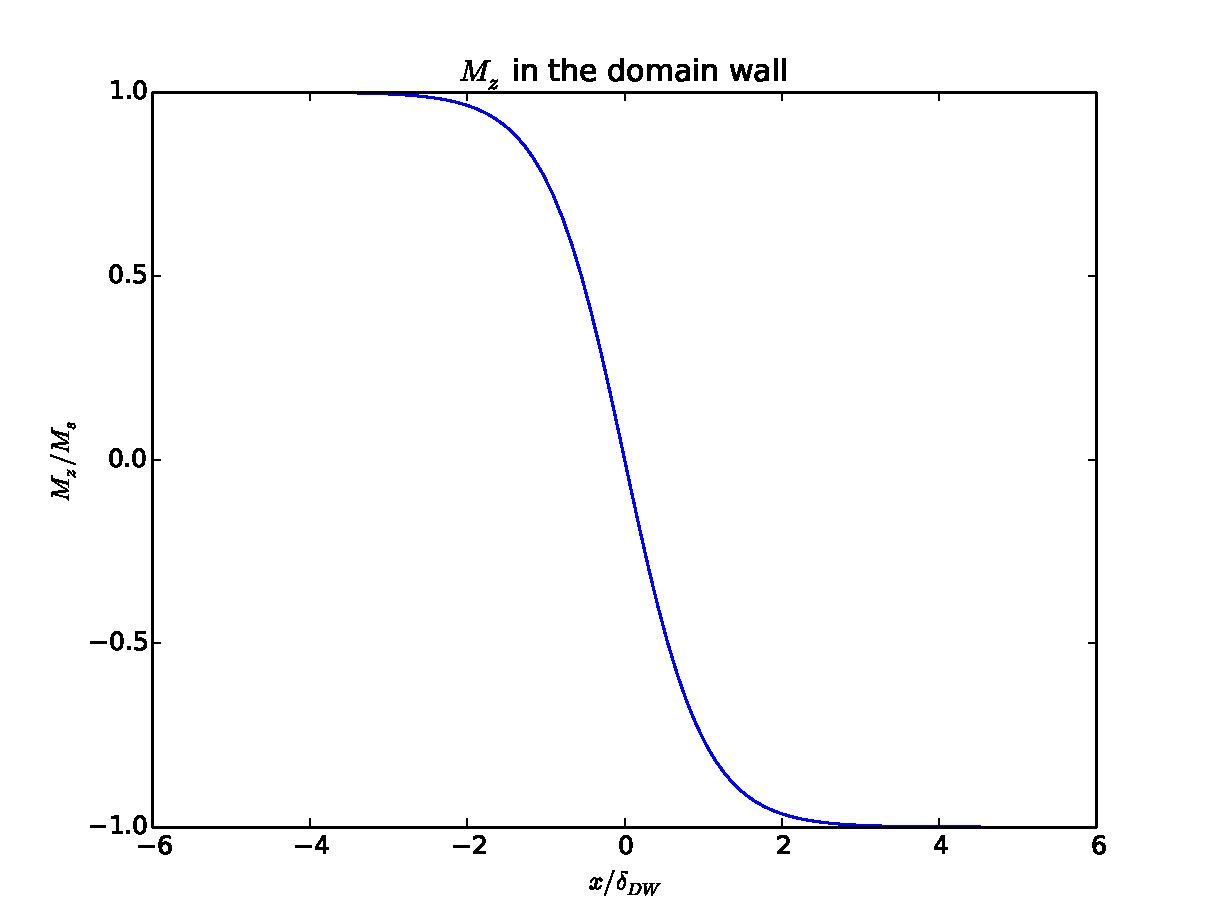
\includegraphics[width=1.0\linewidth]{Figures/BlochWallMz}
  \caption{}
\end{subfigure}%
\begin{subfigure}{.5\textwidth}
  \centering
  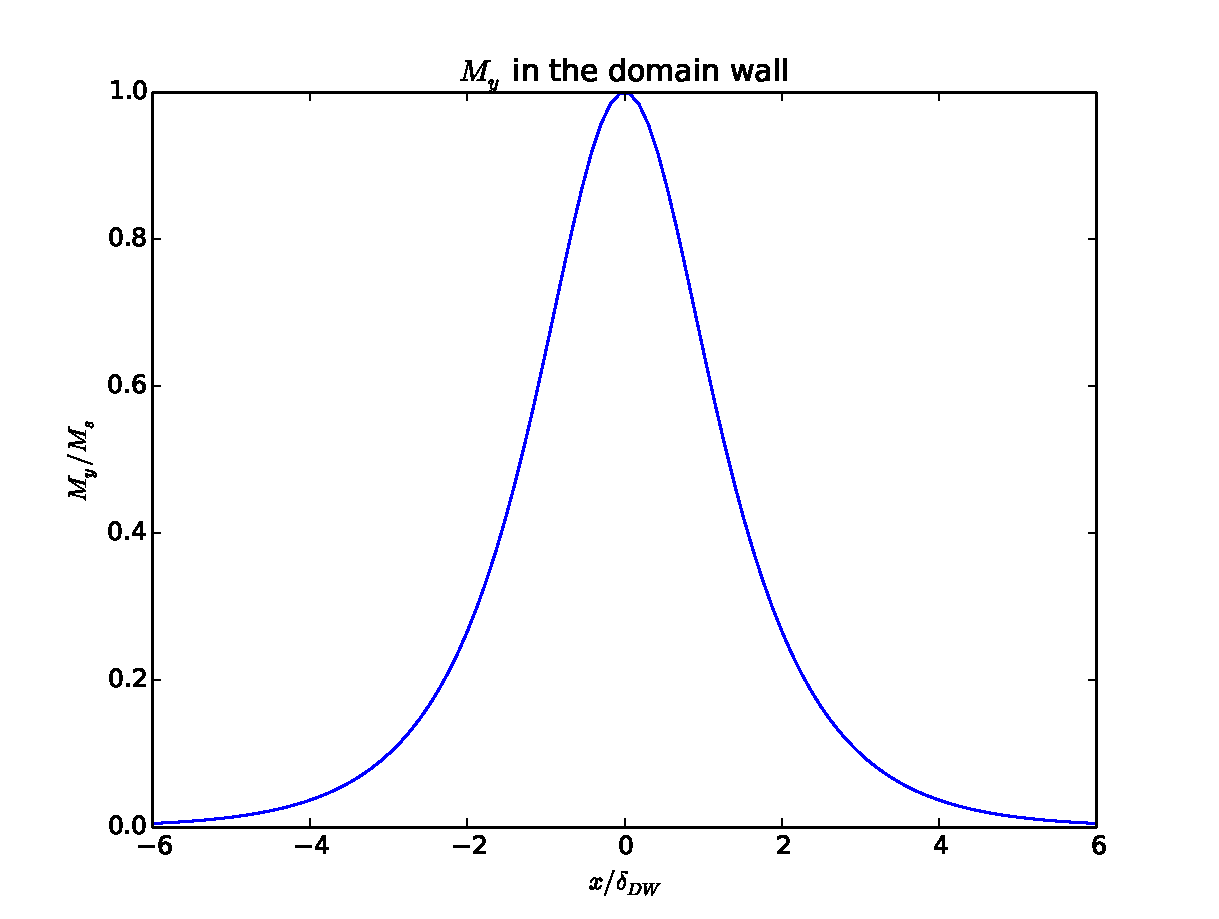
\includegraphics[width=1.0\linewidth]{Figures/BlochWallMy}
  \caption{}
\end{subfigure}
\caption{The magnetization component in the $z$-direction (a) and in the $y$-direction (b) inside a Bloch domain wall with $X = 0$.}
\label{fig:BlochWall}
\end{figure}
The magnetization components are shown as a function of $x/\delta_{DW}$ in Figure \ref{fig:BlochWall}. This type of domain wall where the magnetization rotates out of the plane that is parallel to the magnetization in the domains is known as a Bloch wall \cite{Bloch1932}. In the derivation of the expression for the Bloch wall we chose this direction of rotation as this magnetization structure did not create any magnetic volume charges $-\nabla\cdot\vec{M}$. To minimize the demagnetization energy we want to avoid both magnetic volume and surface charges. We see that surface charges can be created by the Bloch domain wall if the plane the domains are in is parallel and close to the surface of the magnet. This is because the Bloch domain wall rotates out of that plane, giving a component that is normal to the magnet's surface. If the domain wall is far away from a surface, however, there will not be any creation of a surface charge. Bloch domain walls are the most common domain walls in bulk materials. This is because of the thickness of the material makes it more energetically favorable to avoid volume charges than surface charges.

\subsection{N\'{e}el walls}
If the magnetic material has a large surface area, such as thin films, it may be more energetically favorable to avoid surface charges than to avoid volume charges. To have a domain wall that does this, we must require that the magnetization in the domain wall rotates in the plane of the domains, unlike the Bloch domain wall where the magnetization rotates out of that plane. If we look at a similar example as in the derivation of the Bloch domain wall, we must have a magnetization that rotates in the $xz$-plane rather than the $yz$-plane, as we let the $y$-direction be the direction normal to the magnet's surface. The easy axis in the material is kept to be along the $z$-axis. The energy expressions and the equation for $\theta (x)$ are exactly the same as for the Bloch domain wall, the only difference is that instead of forcing $\phi$ to be $\pi/2$ to avoid magnetic volume charges, we force $\phi$ to be 0 to let the $M_y$ component be 0 and thereby avoiding generating magnetic surface charges. The function $\theta(x)$ is therefore exactly the same as for the Bloch domain wall, given by \eqref{eq:thetaBloch}. The magnetization vector changes, however, from being $\vec{M} = M_s(0, \sin\theta, \cos\theta)$ for the Bloch domain wall to being $\vec{M} = M_s(\sin\theta, 0, \cos\theta)$ for our current domain wall. In other words, the magnetization component in the $x$- and $y$-directions switch. The magnetization therefore looks the same as in Figure \ref{fig:BlochWall}, with $M_y \rightarrow M_x$ and $M_y=0$. This type of domain wall where the magnetization rotates in the plane of the domain magnetization is known as a N\'{e}el domain wall. This type of domain wall does not generate any surface charges, assuming the domains are parallel to the surface of the magnet, but generates magnetic volume charges as the divergence of the magnetization is not zero. We can calculate the magnetic volume charge that the N\'{e}el wall generates:
\begin{align}
\nonumber\rho_M &= -\nabla\cdot\vec{M}(x) \\
\nonumber&= -M_s \frac{\partial}{\partial x} \sin \theta(x) \\
&= \frac{M_s}{\delta_{DW}}\frac{\tanh\frac{x-X}{\delta_{DW}}}{\cosh\frac{x-X}{\delta_{DW}}}.
\end{align}
\begin{figure}[h!]
\begin{center}
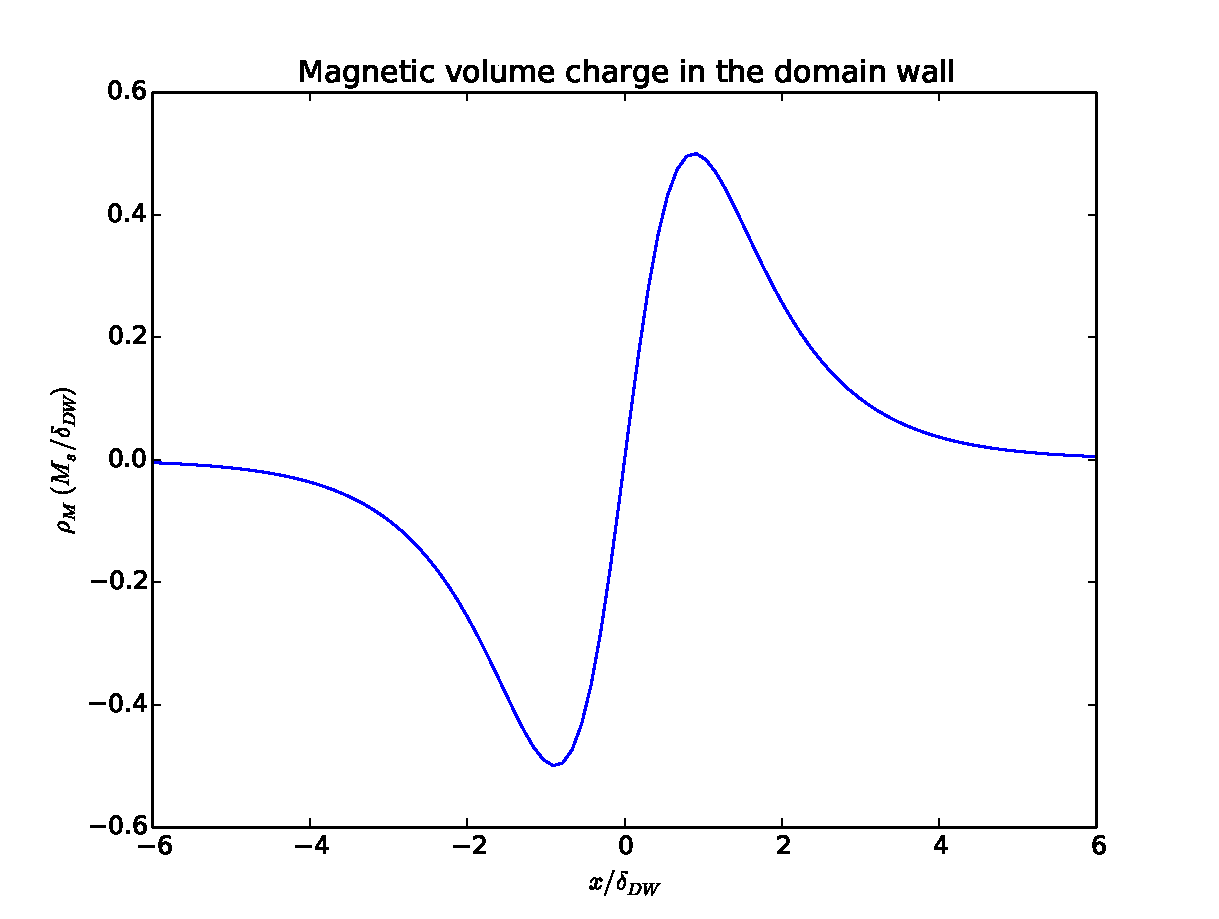
\includegraphics[width=0.8\textwidth]{Figures/MagneticVolumeCharge.pdf} 
\caption{The distribution of the magnetic volume charge inside a N\'{e}el domain wall.}
\label{fig:magVolumeCharge} 
\end{center}
\end{figure}
This magnetic volume charge distribution is shown in Figure \ref{fig:magVolumeCharge}. It is antisymmetric, and the total magnetic volume charge is zero. The magnetic volume charge therefore acts as a magnetic dipole.

\subsection{Domain wall width and energy}
To find the width of the domain wall separating the two domains, we need to define where the domain begins, as $M_z$ only approaches $\pm M_s$ asymptotically. One way to do that is to find the value of $x$ where $M_z$ has reached a certain percentage of $M_s$, and then let the domain wall width be twice that value as the domain wall is antisymmetric around $x=0$. This can be done by inverting \eqref{eq:BlochMagZ}. We then find that the width of the domain wall $\Delta_{DW}$ is
\begin{align}
\Delta_{DW} = 2\delta_{DW}\ln\sqrt{\frac{M_s+|M_z|}{M_s-|M_z|}}.
\end{align}
If we let the domains begin when $|M_z| = 0.99\cdot M_s$, we get that the domain wall width is $\Delta_{DW} \approx 5.3 \cdot \delta_{DW}$. This is true for both the Bloch domain walls and N\'{e}el domain walls we have derived earlier. Remembering that the characteristic length $\delta_{DW}$ was defined as $\delta_{DW} = \sqrt{A/K}$, we see that the width of the domain wall is determined by what is the more dominating term in the energy; the exchange interaction or the anisotropy. If the exchange interaction influences the energy much more than the anisotropy, the domain wall becomes very wide, as the magnetization wants to change very slowly to reduce the exchange energy. If the material is isotropic, meaning $K\rightarrow0$, the width of the domain wall becomes infinite. This is because when there is no anisotropy the stable energy state is when all spins are aligned. Anisotropy is therefore necessary for the existence of domain walls in this model where the demagnetization energy is not explicitly accounted for.

Even though domain walls are stable states, they have an energy cost from the exchange interaction and the anisotropic energy compared to uniform domains. This energy cost can be found by first rewriting \eqref{eq:BlochEnergy} to remove the constant energy in the domains, and then plug in our domain wall solutions to do the integral over the domain wall. The integrand is $-K$ in our domains ($\theta = 0$ and $\theta = \pi$), so we add a constant term of $K$ to the integrand to let the domains have no energy contributions from anisotropy or the exchange interaction. We then integrate to find the energy per domain wall area:
\begin{align}
\nonumber\frac{\textrm{d} E_{DW}}{\textrm{d} A} &= \int_{-\infty}^{\infty} \d x \left(\frac{A}{M_s^2}(\frac{\partial}{\partial x}\vec{M}(x))^2 - K \cos ^2 \theta (x) + K\right) \\
\nonumber&= \int_{-\infty}^{\infty} \d x \left(\frac{A}{\delta_{DW}^2}\frac{1}{\cosh^2\frac{x}{\delta_{DW}}} + K \frac{1}{\cosh^2\frac{x}{\delta_{DW}}}\right) \\
&= 4K\delta_{DW} = 4\sqrt{AK}.
\end{align}

\section{Domain wall dynamics} \label{sec:DWDynamics}
Domain walls can be moved by applying an electric current to the magnetic material. This is done either by a momentum transfer or spin transfer between the local electrons and the conduction electrons. A momentum transfer would correspond to actual movement of the electrons in the domain wall, so that the domain wall moves with them, while a spin transfer corresponds to a shift in the local magnetization due to the exchange interaction with the conduction electrons. Here only the domain wall moves, and the position of the electrons in the domain wall is unchanged. For domain walls where the magnetization does not change abruptly, so that the spin of the conduction electron can follow the local magnetization more or less adiabatically, the spin transfer effect will be the dominant cause of the domain wall motion \cite{KohnoTatara-04}. 

\subsection{Spin-transfer torque}
The adiabatic spin-transfer torque is a consequence of conservation of angular momentum, or spin. As the spin of the conduction electron follows the variation in the magnetization in the domain wall, there will be a torque acting on the local magnetization in the opposite direction of the rotation of the itinerant spin. This is simply Newton's third law; for the torque acting on the itinerant electron moving through the local magnetization, there will be an equal and opposite torque acting on the local magnetization. When this process is adiabatic the total spin of the local and itinerant electrons is conserved. There is also a non-adiabatic spin-transfer torque, which occurs when the itinerant electron does not move completely adiabatically through the magnet. 

To model the spin-transfer torque acting on the local magnetization in the magnet, we mainly follow the derivation by Zhang and Li \cite{ZhangLi-04}. The spin density of the itinerant electrons in the applied current can in general be written as
\begin{align}
\label{eq:mag_current}
\vec{m} = \langle \vec{s} \rangle = \frac{m_0}{M_s}\vec{M} + \delta\vec{m}.
\end{align}
Here we have split the magnetization into two components, the first of which is parallel to the local magnetization $\vec{M}$, and the second component $\delta\vec{m}$ which  is perpendicular to the local magnetization. It is assumed that the component parallel to the local magnetization is much larger than the perpendicular component, as the magnetization of the itinerant electrons follows the local magnetization mostly adiabatically. One should also note that $m_0/M_s \ll 1$ as the itinerant current is not near being saturated. The time evolution of the itinerant spins are given by the continuity equation
\begin{align}
\label{eq:spin_continuity}
\frac{\partial \vec{s}}{\partial t} + \nabla \hat{J} = \frac{1}{i\hbar} \left[ \vec{s}, H_{sd} \right] - \Gamma(\vec{s}),
\end{align}
with $\hat{J}$ being the spin current operator and $\Gamma(\vec{s})$ describes the relaxation of the non-adiabatic spins. The s-d interaction Hamiltonian $H_{sd}$ describes the exchange energy between the itinerant spin $\vec{s}$ and the local spin $\vec{S}$,
\begin{align}
H_{sd} = -J \vec{s} \cdot \vec{S} = -J \vec{s} \cdot (-\frac{S}{M_s} \vec{M}).
\end{align}
The commutator in \eqref{eq:spin_continuity} can be approximated by
\begin{align}
\frac{1}{i\hbar} \left[ \vec{s}, H_{sd} \right] = - \frac{1}{i\hbar} \left[ H_{sd}, \vec{s} \right] \approx -\frac{1}{i\hbar}\sum_{i, j} \frac{\textrm{d} H_{sd}}{\textrm{d} s_i}\left[ s_i, s_j \right]
\end{align}
in the semi-classical limit \citep{kruger2006current}. Using that the dimensionless spins can be written on the form $s_i = \sigma_i/2$, with $\sigma_i$ being the Pauli matrices, we use the commutation relation between the Pauli matrices to find that
\begin{align}
\left[ s_i, s_j \right] = \sum_k i\varepsilon_{ijk} s_k.
\end{align}
Combining this with $\frac{\textrm{d} H_{sd}}{\textrm{d} s_i} = -JS_i$, we get that
\begin{align}
\frac{1}{i\hbar} \left[ \vec{s}, H_{sd} \right] \approx - \frac{1}{i\hbar} \sum_{i,j, k} (-J S_i) i\varepsilon_{ijk}  s_k = -\frac{J}{\hbar} \vec{S} \times \vec{s}.
\end{align}
Using this result, and letting the operators become their expectation values, we get the continuity equation for $\vec{m}$:
\begin{align}
\label{eq:spindensity_continuity}
\frac{\partial \vec{m}}{\partial t} + \nabla \langle\hat{J}\rangle = -\frac{J S}{\hbar M_s} \vec{m} \times \vec{M} - \langle\Gamma(\vec{m})\rangle.
\end{align}
The first term on the right hand side is a torque acting on $\vec{m}$ from the interaction between $\vec{m}$ and $\vec{M}$. By Newton's third law there will be an equal and opposite torque acting on the local magnetization $\vec{M}$, so that the spin-transfer torque becomes
\begin{align}
\label{eq:STT}
\vec{T}_{STT} = -\frac{J S}{\hbar M_s} \vec{M} \times \vec{m} = -\frac{J S}{\hbar M_s} \vec{M} \times \delta\vec{m}
\end{align}
To determine the spin-transfer torque we must find an expression for $\delta\vec{m}$. This is done by solving \eqref{eq:spindensity_continuity}. To do that one has to make some basic assumptions. We assume that the relaxation of the non-adiabatic spins is proportional to the non-adiabatic component of $\vec{m}$. By letting the average spin-flip relaxation time be defined by $\tau_{sf}$, the last term in \eqref{eq:spindensity_continuity} becomes $\langle\Gamma(\vec{m})\rangle \approx \delta\vec{m}/\tau_{sf}$. 

The spin current density is a tensor of rank 2, defined by the vectors that describe the charge flow and the spin of the conduction electrons. As the spin and magnetization of an electron are anti-parallel, the adiabatic spin current density can then be written as
\begin{align}
\langle \hat{J}_{\textrm{adiabatic}} \rangle = -\frac{\mu_B P}{e} \vec{j}_e \otimes \frac{\vec{M}}{M_s}.
\end{align}
The factor $P$ describes the portion of the conduction electrons that are polarized in the direction of the local electrons, and $e$ is the elementary charge. The factors $\mu_B$ and $e$ are included to get the correct units. If one assumes a uniform charge current density $\vec{j}_e$, and that the non-adiabatic spin current is negligible (which is alright if the domain wall width is much greater than the transport length scale, see \cite{ZhangLi-04}), the spin current term becomes
\begin{align}
\nabla \langle \hat{J} \rangle = \nabla \left(-\frac{\mu_B P}{e} \vec{j}_e \otimes \frac{\vec{M}}{M_s}\right) = -\frac{\mu_B P}{e M_s} (\vec{j}_e \cdot \nabla) \vec{M}.
\end{align}
Remembering that we have an adiabatic component of $\vec{m}$ that is much greater than the non-adiabatic component $\delta\vec{m}$, we ignore the term $\frac{\partial \delta\vec{m}}{\partial t}$, which is necessary to obtain an analytical solution of $\delta \vec{m}$. Combining all of these assumptions and inserting them into \eqref{eq:spindensity_continuity}, the equation becomes 
\begin{align}
\label{eq:dm_implicit}
\frac{m_0}{M_s}\frac{\partial \vec{M}}{\partial t} - \frac{\mu_B P}{e M_s} (\vec{j}_e \cdot \nabla) \vec{M} = -\frac{1}{\tau_{ex} M_s} \delta\vec{m} \times \vec{M} - \frac{\delta\vec{m}}{\tau_{sf}},
\end{align}
where we have introduced the spin exchange relaxation timescale $\tau_{ex} = \hbar/JS$. This equation can be solved explicitly for $\delta\vec{m}$ in the same manner that we transformed the LLG equation from the implicit form to the explicit Landau--Lifshitz form. To do that we took the cross product of the equation with $\vec{M}$ from the left. Doing that, we find that the term $\delta\vec{m}\times\vec{M}$ can be written linearly in $\delta\vec{m}$ as
\begin{align}
\delta\vec{m} \times \vec{M} = \tau_{sf} \left(\frac{m_0}{M_s} \vec{M} \times \frac{\partial \vec{M}}{\partial t} - \frac{\mu_B P}{e M_s} \vec{M}\times((\vec{j}_e\cdot\nabla)\vec{M}) + \frac{M_s}{\tau_{ex}} \delta\vec{m}\right),
\end{align}
as $\vec{M} \times (\delta\vec{m}\times\vec{M}) = M_s^2\delta\vec{M}$. Inserting this result back into \eqref{eq:dm_implicit} and solving for $\delta\vec{m}$, we find the explicit expression
\begin{align}
\label{eq:dm_explicit}
\delta\vec{m} = \frac{\tau_{ex}}{1+\xi^2}\left(-\frac{m_0\xi}{M_s}\frac{\partial \vec{M}}{\partial t} + \frac{\xi \mu_B P}{e M_s}(\vec{j}_e\cdot\nabla)\vec{M} - \frac{m_0}{M_s^2}\vec{M}\times \frac{\partial \vec{M}}{\partial t} + \frac{\mu_B P}{e M_s^2}\vec{M}\times((\vec{j}_e\cdot\nabla)\vec{M})\right),
\end{align}
with $\xi$ being defined as the ratio $\xi = \tau_{ex}/\tau_{sf}$. Inserting this into the expression for the spin-transfer torque given in \eqref{eq:STT}, we find that the spin-transfer torque $\vec{T}_{STT}$ as a function of the local magnetization $\vec{M}(\vec{r}, t)$ and the charge current density $\vec{j}_e$ is 
\begin{align}
\nonumber\vec{T}_{STT} = &\frac{1}{1+\xi^2} \bigg(\frac{m_0\xi}{M_s}\vec{M}\times\frac{\partial \vec{M}}{\partial t} - \frac{\xi\mu_B P}{e M_s^2}\vec{M}\times(\vec{j}_e\cdot\nabla)\vec{M} \\
&- \frac{m_0}{M_s} \frac{\partial \vec{M}}{\partial t} - \frac{\mu_B P}{e M_s^3} \vec{M}\times (\vec{M}\times(\vec{j}_e\cdot\nabla)\vec{M})\bigg).\label{eq:STT_final}
\end{align}
Here we have used that $\vec{M}\times(\vec{M}\times\frac{\partial \vec{M}}{\partial t}) = -M_s^2\frac{\partial \vec{M}}{\partial t}$ as $\vec{M}\cdot\frac{\partial \vec{M}}{\partial t} = 0$, and that $\tau_{ex} = \hbar/JS$. Using this result we can extend the LLG equation in \eqref{eq:LLG_implicit} to also include the spin-transfer torque effects from the charge current, by inserting $\vec{T}_{STT}$ into the right hand side. Looking at the implicit LLG equation we see that we already have terms that go as $\frac{\partial \vec{M}}{\partial t}$ and $\vec{M}\times\frac{\partial \vec{M}}{\partial t}$. These terms in the spin-transfer torque $\vec{T}_{STT}$ can therefore be incorporated into the LLG equation by redfining the gyromagnetic ratio $\gamma$ and the damping parameter $\eta$. If one inserts the terms in $\vec{T}_{STT}$ that do not depend on the current into \eqref{eq:LLG_implicit}, one finds that by letting
\begin{align}
\beta &= \frac{m_0}{M_s}\frac{1}{1+\xi^2}, \\
\gamma ' &= \frac{\gamma}{1+\beta}, \\
\eta ' &= \eta + \frac{\xi\beta}{\gamma},
\end{align}
the LLG equation keeps its original form. As $m_0\ll M_s$, we also get $\beta \ll 1$, and so the corrections to $\gamma$ and $\eta$ are relatively small. The real impact from the spin-transfer torque comes from the terms dependent on the current. Including these terms the extended LLG equation becomes
\begin{align}
\label{eq:LLG_current}
\frac{\textrm{d} \vec{M}}{\textrm{d} t} = -\gamma ' \vec{M} \times (\vec{H}_{eff} - \eta '\frac{\textrm{d} \vec{M}}{\textrm{d} t}) - \frac{b_J}{M_s^2} \vec{M}\times (\vec{M}\times(\hat{j}_e\cdot\nabla)\vec{M})) - \frac{c_J}{ M_s}\vec{M}\times(\hat{j}_e\cdot\nabla)\vec{M},
\end{align}
with $\hat{j}_e$ being the unit vector along the electring current, and $b_J$ and $c_J$ being defined by
\begin{align}
\label{eq:bJ} b_J &= \frac{1}{1+\xi^2} \frac{\mu_B j_e P}{e M_s}, \\
c_J &= \xi b_J.
\end{align}
By looking at the directions of the $b_J$ and $c_J$ terms in \eqref{eq:LLG_current}, one sees that the $b_J$ term is parallel to the direction along which the local magnetization varies, and that the $c_J$ term is perpendicular to the plane that the local magnetization and the change in the local magnetization constitute. If one considers the magnetization of a N\'{e}el wall in the $x$-direction and a flow of electrons in the positive $x$-direction, the direction of the charge current becomes $\hat{j}_e = -\hat{x}$. The minus sign is because there is a flow of negative charges. If one lets the magnetization of the N\'{e}el wall point along $\hat{z}$ at $x = -\infty$, and along $-\hat{z}$ at $x = \infty$, and let the magnetization of the conduction electrons follow the local magnetization mostly adiabatically, the $b_J$ term will point in the opposite direction of $\frac{\partial \vec{M}}{\partial x}$ and the $c_J$ term will point along $-\hat{y}$. The $b_J$ term is therefore known as the adiabatic spin-transfer torque as it adjusts the local magnetization in the opposite direction of the adiabatic motion of the magnetization of the conduction electrons. Similarly the $c_J$ term is known as the non-adiabatic spin-transfer torque as it adjusts the local magnetization perpendicularly to the adiabatic motion of the magnetization of the conduction electrons. 

The form of the extended LLG equation in \eqref{eq:LLG_current} is implicit in $\frac{\textrm{d} \vec{M}}{\textrm{d} t}$. Like the implicit LLG equation, it can be transformed into an explicit form by taking the cross product of it with $\vec{M}$, to get a linear expression for $\vec{M}\times\frac{\textrm{d} \vec{M}}{\textrm{d} t}$ in $\frac{\textrm{d} \vec{M}}{\textrm{d} t}$. It is then easy to show that by choosing
\begin{align}
\eta' &= \frac{\alpha}{\gamma ' M_s}, \\
\tilde{\gamma}' &= \frac{\gamma '}{1+\alpha^2},
\end{align}
with $\alpha$ being a dimensionless damping constant like in the Landau--Lifshitz equation, we get the explicit form of the extended LLG equation:
\begin{align}
\nonumber \frac{\partial \vec{M}}{\partial t} = &-\tilde{\gamma}' \vec{M} \times  \left(\vec{H}_{eff} + \frac{\alpha}{M_s} \vec{M}\times \vec{H}_{eff}\right) \\ 
&- \frac{(1+\alpha\xi) b_J}{M_s^2(1+\alpha^2)} \vec{M}\times (\vec{M}\times(\hat{j}_e\cdot\nabla)\vec{M})) - \frac{(\xi-\alpha)b_J}{ M_s(1+\alpha^2)}\vec{M}\times(\hat{j}_e\cdot\nabla)\vec{M}.
\label{eq:LLG_current_explicit}
\end{align}
From this equation one can easily see that there will always be an adiabatic spin-transfer torque when a charge current is propagating through a domain wall, but there will only be a torque perpendicular to $\vec{M}$ and $\frac{\partial\vec{M}}{\partial x}$ if $\xi \neq \alpha$. As $\xi = \tau_{ex}/\tau_{sf}$, with $\tau_{ex}$ being a time scale in the exchange interaction and $\tau_{sf}$ being an average relaxation time of the non-adiabatic electrons, $\xi$ describes a dimensionless damping parameter for the conduction electrons \cite{kruger2006current}. There will therefore be an out-of-plane torque when the damping of the local and the conduction electron spins are different, with the plane here being spanned by $\vec{M}$ and $\frac{\partial\vec{M}}{\partial x}$. This out-of-plane torque causes a rotation of the domain wall, as one of the spins will relax faster than the other.

\subsection{Domain wall motion}
\subsubsection{Advection}
In the simplest case when the damping of the itinerant and local spins are equal ($\xi = \alpha$), \eqref{eq:LLG_current_explicit} can be reduced considerably to
\begin{align}
\label{eq:dw_advection}
\frac{\partial \vec{M}(\vec{r}, t)}{\partial t} - b_J(\hat{j}_e\cdot\nabla) M(\vec{r}, t) = 0.
\end{align}
To get this one assumes that the local magnetization is in equilibrium when the current is applied, so that the terms including the effective field vanish. One also assumes a homogeneous material so that $\vec{M}\cdot(\hat{j}_e\cdot\nabla)\vec{M} = 0$ as $|\vec{M}(\vec{r}, t)| = M_s$ is a constant, meaning $\vec{M}\times (\vec{M}\times(\hat{j}_e\cdot\nabla)\vec{M})) = -M_s^2(\hat{j}_e\cdot\nabla)\vec{M}$. Comparing \eqref{eq:dw_advection} to the advection equation for a vector field $\vec{M}(\vec{r}, t)$ with an incompressible flow $\vec{v}$,
\begin{align}
\label{eq:advection}
\frac{\partial \vec{M}(\vec{r}, t)}{\partial t} + (\vec{v}\cdot\nabla) \vec{M}(\vec{r}, t) = 0,
\end{align}
one sees that the domain wall moves with a velocity $\vec{v} = -b_J \hat{j}_e$. As $\hat{j}_e$ points in the opposite direction of the electron flow, the domain wall moves in the same direction as the electrons with a speed $b_J$. The solution of the advection equation is $\vec{M}(\vec{r} - \vec{v} \cdot (t - t_0), t_0)$, with $\vec{M}(\vec{r}, t_0)$ having to satisfy the LLG equation per our assumptions. The simple case described by \eqref{eq:dw_advection} is then just an advection of a domain wall, such as a Bloch or N\'{e}el wall.

\subsubsection{Spin-transfer torque}
To solve the extended LLG equation, it will be useful to write the equation in spherical coordinates and use the solution for $\theta(x)$ we found earlier in \eqref{eq:thetaBloch}. To do this, we write the vectors in terms of their spherical components. An infitesimal change in the magnetization can then be written as
\begin{align}
\label{eq:dm_spherical}
\d {\vec{M}} = \d M_s \hat{r} + M_s \d {\theta} \hat{\theta} + M_s\sin\theta\d {\phi} \hat{\phi},
\end{align}
which is easily seen from the geometry. Using that $\frac{\textrm{d} M_s}{\textrm{d} t} = 0$, we then find
\begin{align}
\frac{\partial \vec{M}}{\partial t} = M_s
\begin{pmatrix}
0 \\ 
\dot{\theta} \\ 
\sin\theta\dot{\phi}
\end{pmatrix}.
\end{align}
Note here that the first component in the vector is the radial component, the second is the component along $\hat{\theta}$, and the last component is along $\hat{\phi}$. Using the definition of the effective field, we find in a similar manner that
\begin{align}
\vec{H}_{eff} = -\frac{1}{\mu_0} \frac{\delta \epsilon}{\delta \vec{M}} = -\frac{1}{\mu_0}
\begin{pmatrix}
\frac{\delta \epsilon}{\delta M_s} \\ 
\frac{1}{M_s} \frac{\delta \epsilon}{\delta \theta} \\ 
\frac{1}{M_s\sin\theta} \frac{\delta \epsilon}{\delta \phi}
\end{pmatrix}.
\end{align}
For the current terms in \eqref{eq:LLG_current_explicit}, we note that $(\hat{j}_e\cdot\nabla)$ is a scalar operator, so that $(\hat{j}_e\cdot\nabla)\vec{M} = \sum_i c_i \frac{\textrm{d} \vec{M}}{\textrm{d} x_i}$. Using \eqref{eq:dm_spherical} we then easily see that we can write
\begin{align}
(\hat{j}_e\cdot\nabla)\vec{M} = M_s
\begin{pmatrix}
0 \\ 
(\hat{j}_e\cdot\nabla)\theta \\ 
\sin\theta(\hat{j}_e\cdot\nabla)\phi
\end{pmatrix},
\end{align}
where we have also used that $\frac{\textrm{d} M_s}{\textrm{d} x_i} = 0$. The scalar operator $(\hat{j}_e\cdot\nabla)$ can be kept in cartesian coordinates, as we can have $\theta$ and $\phi$ as a function of $x$, $y$ and $z$. Finally, we use again that $\vec{M}\times (\vec{M}\times(\hat{j}_e\cdot\nabla)\vec{M})) = -M_s^2(\hat{j}_e\cdot\nabla)\vec{M}$. Combining all of this into \eqref{eq:LLG_current_explicit} and calculating the cross products yields the extended LLG equation in spherical coordinates:
\begin{align}
\nonumber \begin{pmatrix}
0 \\ \dot{\theta} \\ \sin\theta\dot{\phi}
\end{pmatrix} =
&\frac{\tilde{\gamma}'}{\mu_0 M_s}
\begin{pmatrix}
0 \\ -\frac{1}{\sin\theta} \frac{\delta \epsilon}{\delta \phi} \\ \frac{\delta \epsilon}{\delta \theta}
\end{pmatrix} - \frac{\tilde{\gamma}' \alpha}{\mu_0 M_s} 
\begin{pmatrix}
0 \\ \frac{\delta \epsilon}{\delta \theta} \\ \frac{1}{\sin\theta} \frac{\delta \epsilon}{\delta \phi}
\end{pmatrix} + \frac{(1+\xi\alpha)b_J}{1+\alpha^2}
\begin{pmatrix}
0 \\ (\hat{j}_e\cdot\nabla)\theta \\ \sin\theta(\hat{j}_e\cdot\nabla)\phi
\end{pmatrix} \\
&+\frac{(\xi-\alpha)b_J}{1+\alpha^2}
\begin{pmatrix}
0 \\ \sin\theta(\hat{j}_e\cdot\nabla)\phi \\ -(\hat{j}_e\cdot\nabla)\theta
\end{pmatrix}.
\label{eq:LLG_current_explicit_spherical}
\end{align}
The radial equation is trivial, but we have two equations in $\theta$ and $\phi$. Now we use this equation to look at a similar case as the N\'{e}el wall described in the last section. We consider a material with an easy axis along the $z$-axis and a hard axis along the $y$-axis. The anisotropic energy density can then be written as
\begin{align}
\nonumber \epsilon_A &= K_{\perp} \left(\frac{\vec{M}\cdot\hat{y}}{M_s}\right)^2 - K \left(\frac{\vec{M}\cdot\hat{z}}{M_s}\right)^2 \\
\nonumber &= K_{\perp}\sin^2\theta\sin^2\phi - K \cos^2\theta \\
&\rightarrow (K + K_{\perp} \sin^2\phi)\sin^2\theta,
\end{align}
where we added a constant shift $K$ in the energy density at the end to simplify the expression. The constants $K$ and $K_{\perp}$ are strictly positive. Comparing this to the anisotropic energy density in the Bloch and N\'{e}el wall calculations previously, we see that they are the same when we let $K \rightarrow K + K_{\perp}\sin^2\phi$. For the N\'{e}el wall case we let $\phi = 0$ previously, but now instead we set $\phi = \phi (t)$. Spatially $\phi$ is a constant, but we allow it to vary in time due to the non-adiabatic spin-transfer torque from the applied current. As $\phi$ does not vary along the 1D chain of local magnetic moments, which we define to be along the $x$-axis as before, the exchange energy is unchanged from the example with the Bloch and N\'{e}el walls discussed earlier. If we let the demagnetization energy be incorporated into the anisotropic energy, the total energy density then becomes
\begin{align}
\label{eq:energydensity_ex_a}
\epsilon = \epsilon_E + \epsilon_A = A \left(\frac{\partial \theta}{\partial x}\right)^2 + K\sin^2\theta + K_{\perp} \sin^2\theta\sin^2\phi
\end{align}
This energy density is the same as the one we solved in the last section, when the substitution of $K$ mentioned above is done. Because of the applied current, the angle $\theta$ is now also a function of time, meaning $\theta = \theta(x,t)$. If we assume that the width of the domain wall does not change in time, we can use \eqref{eq:thetaBloch} to find the shape of the domain wall. The temporal part of $\theta(x,t)$ is made by letting the domain wall center $X$ be a time dependent position $X(t)$. As the length scale $\delta_{DW}$ depends on $K$, we define a new length scale $\lambda$ where we make the substitution for $K$, so that
\begin{align}
\label{eq:lambda_dw}
\lambda = \sqrt{\frac{A}{K + K_{\perp}\sin^2\phi}}.
\end{align}
Together, this gives us
\begin{align}
\label{eq:theta_current}
\theta(x,t) = 2\arctan\left(\exp(\frac{x-X(t)}{\lambda})\right).
\end{align}
We now have the parameters that describe the motion of the domain wall: $X(t)$ and $\phi(t)$. The former describes a translational motion of the domain wall, and the latter describes a rotation. For low energies these parameters fully describe the domain wall dynamics, under the criterion that
\begin{align}
\label{eq:kperp_ll_k}
K_{\perp} \ll K.
\end{align}
If this is not the case, then the $K_{\perp}$ term may lead to deformations of the domain wall, making our assumption of a static shape of the wall invalid. To describe the dynamics of a deformed wall one must use other parameters \cite{TataraKohnoShibata2008}. Assuming that we are in the situation where we can describe the motion of the domain wall with $X(t)$ and $\phi(t)$, we want to rewrite \eqref{eq:LLG_current_explicit_spherical} using these parameters. First we can calculate $\frac{\delta \epsilon}{\delta \theta}$ and $\frac{\delta \epsilon}{\delta \phi}$ by using \eqref{eq:energydensity_ex_a}:
\begin{align}
\frac{\delta \epsilon}{\delta \phi} &= \frac{\partial \epsilon}{\partial \phi} - \frac{\textrm{d}}{\textrm{d} t} \frac{\partial \epsilon}{\partial (\frac{\partial \phi}{\partial t})} = 2K_{\perp}\sin^2 \theta\sin\phi\cos\phi, \\
\frac{\delta \epsilon}{\delta \theta} &= 2(K+K_{\perp} \sin^2 \phi)\sin\theta\cos\theta - 2A\frac{\partial^2 \theta}{\partial x^2}.
\end{align}
We then use \eqref{eq:theta_current}  to find
\begin{align}
\frac{\partial \theta}{\partial x} &=  \frac{1}{\lambda\cosh\frac{x-X}{\lambda}} = \frac{\sin\theta}{\lambda}, \\
\frac{\partial^2 \theta}{\partial x^2} &=  -\frac{\tanh\frac{x-X}{\lambda}}{\lambda^2\cosh\frac{x-X}{\lambda}} = \frac{\sin\theta\cos\theta}{\lambda^2}, \\
\frac{\textrm{d} \theta}{\textrm{d} t} &= -\frac{\dot{X}}{\lambda\cosh\frac{x-X}{\lambda}} = -\frac{\dot{X}}{\lambda}\sin\theta.
\end{align}
This means that $\frac{\delta \epsilon}{\delta \theta} = 0$, which was the condition we used to determine the function $\theta(x)$ in the first place. By using this we can look at how the different terms in the extended LLG equation acts on the domain wall. Looking at \eqref{eq:LLG_current_explicit_spherical}, we see that the equation for $\dot{\theta}$ is decided by the first and third term on the right hand side, as $\frac{\delta \epsilon}{\delta \theta} =  (\hat{j}_e\cdot\nabla)\phi = 0$. The first term is the magnetostatic torque from the effective field, and the third is the adiabatic spin-transfer torque. The in-plane motion of the domain wall is therefore decided by the balance of these two torques; the adiabatic torque will cause a translational movement of the domain wall, which causes the local magnetization to be moved away from equilibrium. This in turn generates an effective field that will attempt to reverse the motion of the domain wall to return to equilibrium. The resulting torques are shown in Figure \ref{fig:Neel_AdSTT_Heff}. In the equation for $\dot{\phi}$ in \eqref{eq:LLG_current_explicit_spherical}, we only get a contribution from the second and fourth terms on the right hand side. These are the Gilbert damping term and the non-adiabatic spin-transfer torque term respectively, which is seen by comparing \eqref{eq:LLG_current_explicit_spherical} to \eqref{eq:LLG_current}. The Gilbert-damping term rotates the N\'{e}el domain wall out of plane, which causes an increase in the anisotropic energy as the hard axis is perpendicular to the domain wall plane. The non-adiabatic spin-transfer torque acts as a counterpart to this rotation, and attempts to rotate the domain wall in the other direction, as seen in Figure \ref{fig:Neel_NonAdSTT_GD}. 
\begin{figure}[h!]
\centering
\begin{subfigure}{\textwidth}
  \centering
  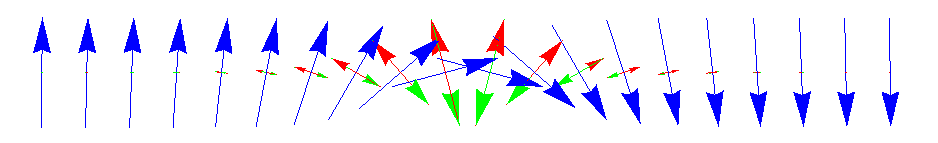
\includegraphics[width=1.0\linewidth]{Figures/NeelWallAdSTTHeff.png}
  \caption{}
  \label{fig:Neel_AdSTT_Heff}
\end{subfigure}
\begin{subfigure}{\textwidth}
  \centering
  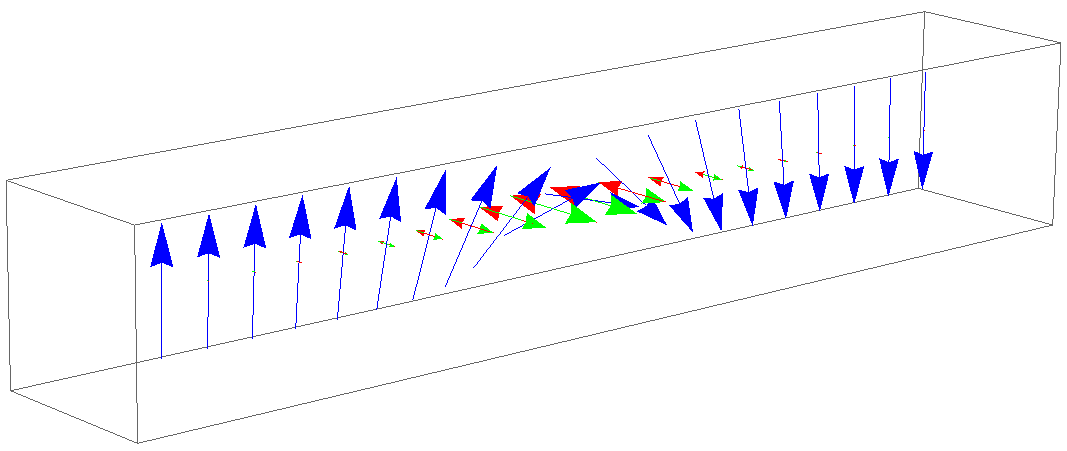
\includegraphics[width=1.0\linewidth]{Figures/NeelWallNonAdSTTGD.png}
  \caption{}
  \label{fig:Neel_NonAdSTT_GD}
\end{subfigure}
\caption{The different torques acting on the initial N\'{e}el domain wall. The blue vectors are the N\'{e}el domain wall magnetization in both figures. In (a) the red vectors represent the adiabatic spin-transfer torque and the green vectors the magnetostatic torque from the effective field. In (b) the red vectors represent the non-adiabatic spin-transfer torque and the green vectors the Gilbert damping torque. The magnitude of the torques are not to scale. The electrons in the applied current move from the domain with spin up to the domain with spin down.}
\end{figure}
If we insert the calculated differentials into \eqref{eq:LLG_current_explicit_spherical} it gives us the two equations
\begin{align}
\begin{pmatrix}
\sin\theta\dot{X} \\ \sin\theta\dot{\phi}
\end{pmatrix}
=
\begin{pmatrix}
\frac{\lambda \tilde{\gamma}'}{\mu_0 M_s} 2 K_{\perp} \sin\theta\sin\phi\cos\phi + \frac{(1+\xi\alpha)b_J}{1+\alpha^2}\sin\theta \\
-\frac{\tilde{\gamma}'\alpha}{\mu_0 M_s}2 K_{\perp} \sin\theta\sin\phi\cos\phi + \frac{(\xi-\alpha)b_J}{\lambda(1+\alpha^2)}\sin\theta
\end{pmatrix}.
\end{align}
We see that $\sin\theta$ is included in all the terms, meaning the domains where $\theta = 0$, $\theta = \pi$ automatically satisfy the equations. As $\sin\theta \neq 0$ except at $x = \pm \infty$, we can safely divide both the equations with $\sin\theta$ when considering the domain wall region:
\begin{align}
\label{eq:xdot_phidot}
\begin{pmatrix}
\dot{X} \\ \dot{\phi}
\end{pmatrix}
=
\begin{pmatrix}
\frac{\lambda \tilde{\gamma}'}{\mu_0 M_s} K_{\perp} \sin2\phi + \frac{(1+\xi\alpha)b_J}{1+\alpha^2} \\
-\frac{\tilde{\gamma}'\alpha}{\mu_0 M_s} K_{\perp} \sin2\phi + \frac{(\xi-\alpha)b_J}{\lambda(1+\alpha^2)}
\end{pmatrix}.
\end{align}
Note that $\lambda$ is a function of $\phi$, but due to the criterion in \eqref{eq:kperp_ll_k} $\lambda$ varies very little as $\phi$ changes. It is therefore alright to assume that $\lambda$ is a constant in the equations. As a cross-check of the validity of \eqref{eq:xdot_phidot} we can see what happens if there is no applied current, meaning $b_J = 0$. We easily see that the domain wall is static if $\dot{X} = \dot{\phi} = 0$, which requires that $\sin2\phi = 0$. This agrees with our solutions earlier, as we have a N\'{e}el wall when $\phi = 0, \pi$ and a Bloch wall when $\phi = \pi/2, 3\pi/2$. Because we are considering a system with a hard axis along the $y$-axis the stable solutions are N\'{e}el walls, so we set $\phi(0) = 0$ in our example. Then we can see that the initial speed of the domain wall is
\begin{align}
\label{eq:Xdot0}
\dot{X}(0) = \frac{1+\xi\alpha}{1+\alpha^2}b_J.
\end{align}
We also have $\dot{\phi}(0) \neq 0$ if $\xi \neq \alpha$, so that the wall rotates slightly. For small currents $j_e$, eventually $\phi(t)$ will obtain a value such that $\dot{\phi}(t) = 0$. If one then solves for $\sin2\phi$ in the second line of \eqref{eq:xdot_phidot} and substitutes into the first line, one then finds that the final domain wall speed becomes
\begin{align}
\label{eq:xdot_undercrit}
\dot{X}(t\rightarrow\infty) = \frac{\xi}{\alpha} b_J.
\end{align}
The final speed of the domain wall is therefore decided by the non-adiabatic spin-transfer torque. Note that this relation is only true up to a certain critical current, as when the current passes a certain threshold, $\dot{\phi} = 0$ is no longer a solution. As $\sin2\phi$ can maximum be 1, we then find that the critical current $j_c$ is given by the relations
\begin{align}
b_{JC} &= \frac{1}{1+\xi^2}\frac{\mu_B P}{e M_s} j_c, \\
j_c &= \frac{\alpha(1+\xi^2)}{\xi-\alpha}\frac{\lambda e \gamma ' K_{\perp}}{\mu_0\mu_B P}. \label{eq:critical_current}
\end{align}
Defining a time scale $T$ for the system,
\begin{align}
T = \frac{\mu_0 M_s}{\tilde{\gamma}' \alpha K_{\perp}},
\end{align}
one can write the equations for $\dot{X}$ and $\dot{\phi}$ as
\begin{align}
\label{eq:xdot_phidot_v2}
\begin{pmatrix}
\dot{X} \\ \dot{\phi}
\end{pmatrix}
=
\begin{pmatrix}
\frac{\lambda}{\alpha T} \sin2\phi + \frac{\lambda}{T}\frac{(1+\xi\alpha)}{\xi - \alpha} \frac{j_e}{j_c} \\
-\frac{1}{T}  \sin2\phi + \frac{1}{T}\frac{j_e}{j_c}
\end{pmatrix}.
\end{align}
It can be shown that the solution of $\phi(t)$ is
\begin{align}
\phi(t) = \arctan\left[\frac{1+\sqrt{(j_e/j_c)^2-1}\tan\left[\sqrt{(j_e/j_c)^2-1}(t/T+C)\right]}{j_e/j_c}\right],
\end{align}
with $C$ being an integration constant. As $\sin2\phi(t)$ is now oscillating in time without reaching a stable value, $\dot{X}$ will always be an oscillating function in time. From now on we will therefore consider the time averaged translational domain wall speed $\langle \dot{X} \rangle$. Using the expression for $\phi(t)$, we find that
\begin{align}
\langle\sin2\phi(t)\rangle = \frac{1}{\frac{\pi T}{\sqrt{(j_e/j_c)^2-1}}} \int_0^{\frac{\pi T}{\sqrt{(j_e/j_c)^2-1}}} \d t \sin2\phi(t) = \frac{j_e}{j_c}-\sqrt{\left(\frac{j_e}{j_c}\right)^2-1}.
\end{align}
Inserting this result into the equation for $\dot{X}$, we find that when $j_e > j_c$
\begin{align}
\label{eq:xdot_av_abovecrit}
\nonumber \langle\dot{X}\rangle &= \frac{\lambda}{T}\left[\frac{1}{\alpha}\left(\frac{j_e}{j_c}-\sqrt{(\frac{j_e}{j_c})^2-1}\hspace{1mm}\right) + \frac{1+\xi\alpha}{\xi-\alpha}\cdot\frac{j_e}{j_c}\right] \\
&= \frac{\xi-\alpha}{1+\alpha^2} \left[\frac{1}{\alpha}\left(\frac{j_e}{j_c}-\sqrt{(\frac{j_e}{j_c})^2-1}\hspace{1mm}\right) + \frac{1+\xi\alpha}{\xi-\alpha}\cdot\frac{j_e}{j_c}\right] b_{JC}.
\end{align}
\begin{figure}[h!]
\centering
\begin{subfigure}{.5\textwidth}
  \centering
  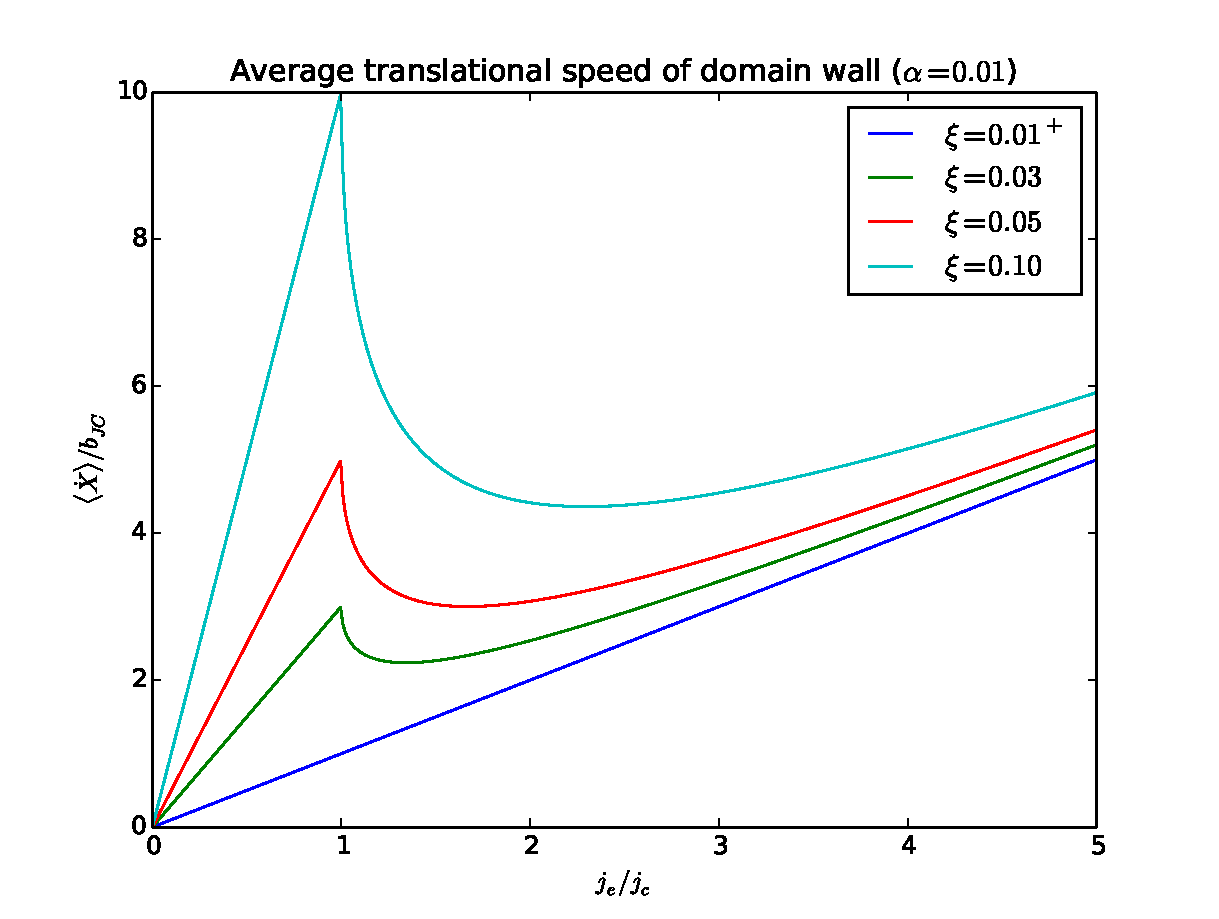
\includegraphics[width=1.0\linewidth]{Figures/walkerBreakdown}
  \caption{}
  \label{fig:walkerBreakdown}
\end{subfigure}%
\begin{subfigure}{.5\textwidth}
  \centering
  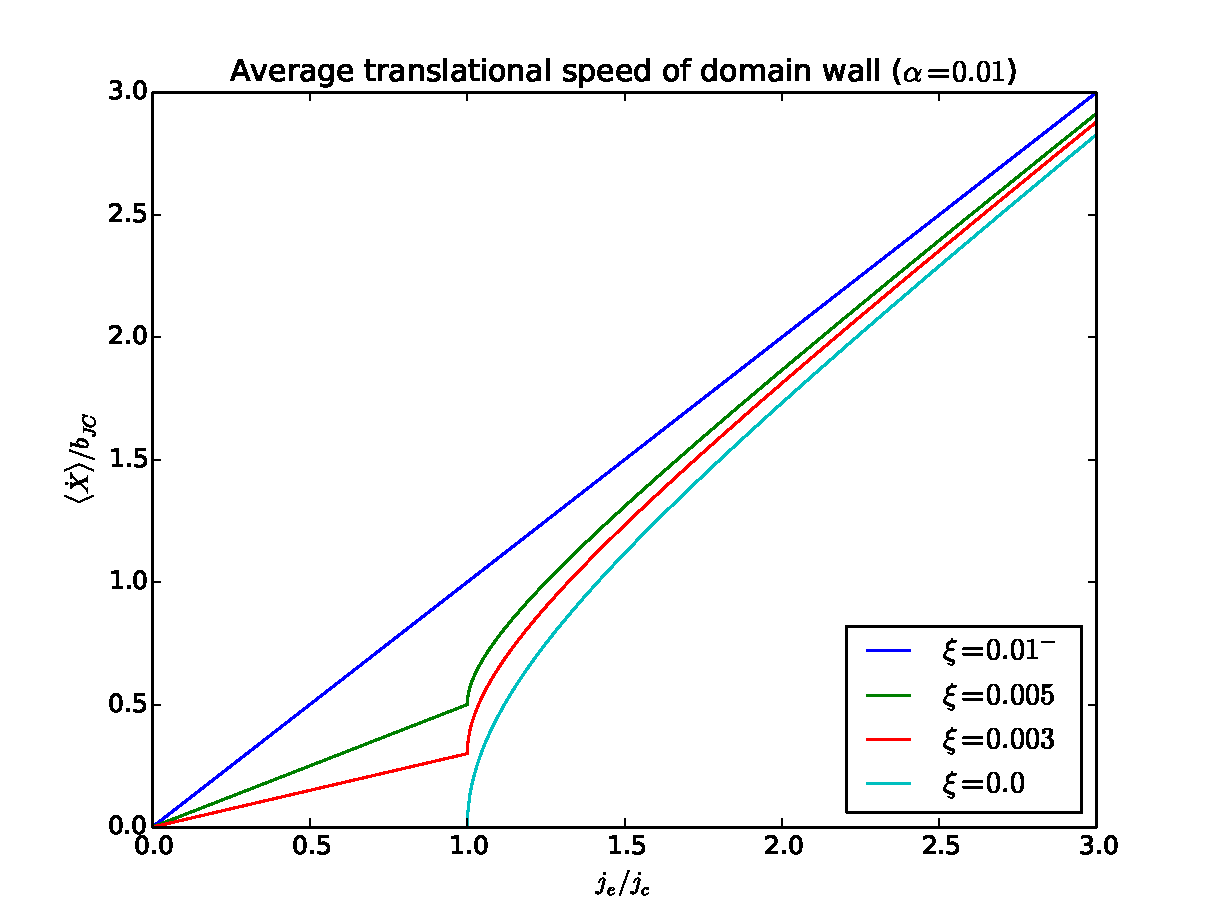
\includegraphics[width=1.0\linewidth]{Figures/criticalCurrentXdot}
  \caption{}
  \label{fig:criticalCurrent}
\end{subfigure}
\caption{The translational speed of the domain wall with a high damping parameter $\xi$ of the itinerant electrons (a) and with a small damping of the itinerant electrons (b) as a function of applied current.}
\label{fig:Xdot_afo_current}
\end{figure}
\begin{figure}[h!]
\begin{center}
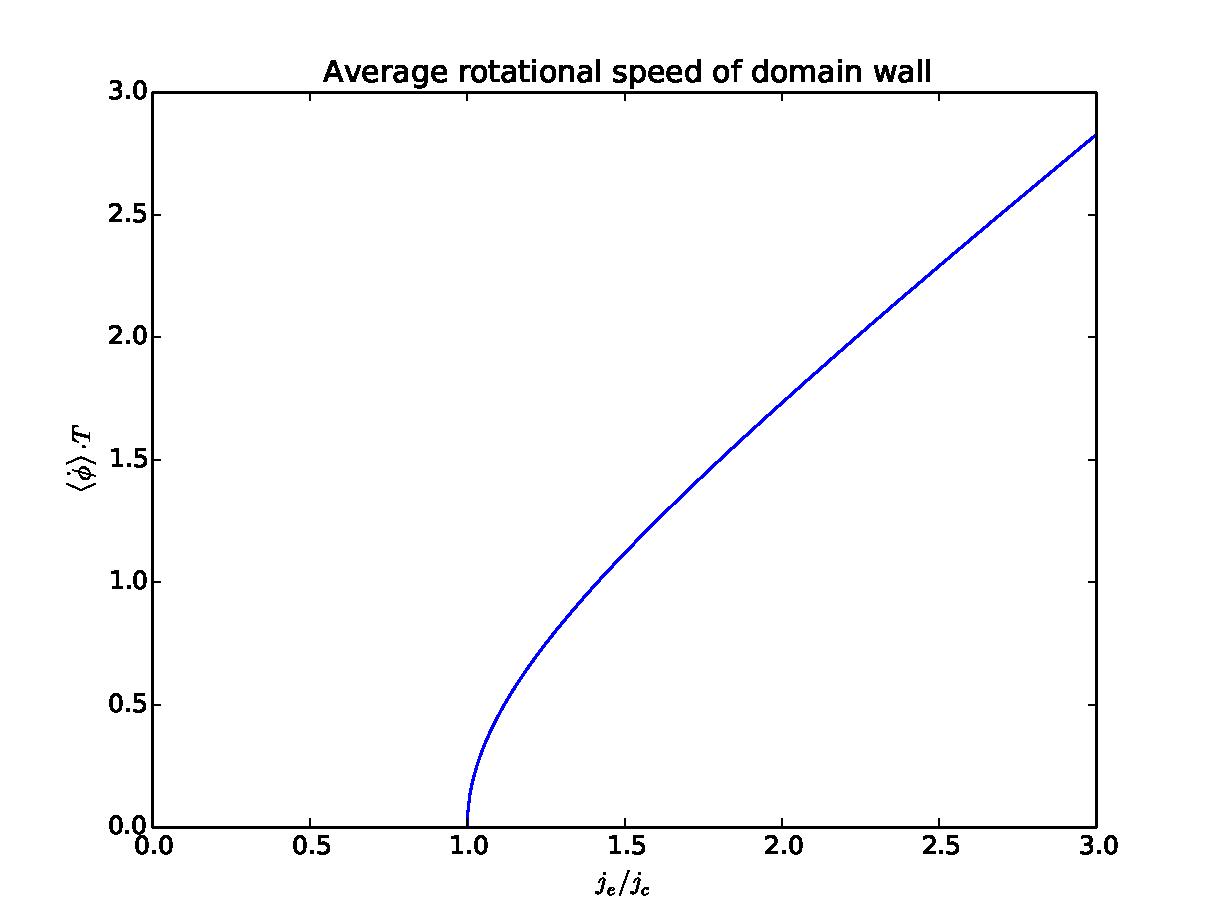
\includegraphics[width=0.8\textwidth]{Figures/criticalCurrentPhidot.pdf} 
\caption{The rotational speed of the domain wall as a function of applied current.}
\label{fig:phidot_afo_current} 
\end{center}
\end{figure}
Combining the results in \eqref{eq:xdot_undercrit} and \eqref{eq:xdot_av_abovecrit} we can plot the translational speed of the domain wall as a function of the applied current for different values of $\xi$, as shown in Figure \ref{fig:Xdot_afo_current}. In Figure \ref{fig:walkerBreakdown} we see a drop in the speed when the applied current exceeds the critical current in the case that $\xi > \alpha$. This is known as a Walker breakdown \cite{SchryerWalker1974}. Above the critical current there is no stable solution of $\phi$, meaning there will be an energy loss to the rotational excitation of the domain wall motion as shown in Figure \ref{fig:phidot_afo_current}. In the limits $j_e/j_c < 1$ and $j_e/j_c \gg 1$ the translational speed $\dot{X}$ is a linear function of $j_e/j_c$. The slope of the function is much steeper for low charge currents, as in this region we do not get any permanent rotational motion of the domain wall. To get a high translational speed at an efficient energy cost through the applied current, it is best to apply a current equal to the critical current. As the correlation between the translational speed of the domain wall and the current is linear, we want a high critical current. It is easily seen from \eqref{eq:critical_current} that the critical current diverges when $\xi \rightarrow \alpha$. If $\xi=\alpha$ there will not be any Walker breakdown. The cause for this is easily seen from Figure \ref{fig:Neel_NonAdSTT_GD}, as when $\xi=\alpha$ the Gilbert damping torque and the non-adiabatic spin-transfer torque cancel each other out, meaning there is no rotational motion of the domain wall. In regards to materialistic properties, one can increase the critical current by making $\lambda K_{\perp}$ large. As 
\begin{align}
\lambda K_{\perp} = \sqrt{\frac{AK_{\perp}}{\frac{K}{K_{\perp}}+\sin^2\phi}},
\end{align}
this is not that easy due to the condition in \eqref{eq:kperp_ll_k}. One can see, however, that the critical current is larger in strongly ferromagnetic materials with large exchange stiffness $A$.

When the itinerant spins have a low damping parameter compared to the local spins ($\xi<\alpha$), the translational speed of the domain wall increases when the applied current is greater than the critical current, as shown in \ref{fig:criticalCurrent}. It is worth noting that the domain wall does not get a final translational speed when the applied current is below the critical current, in the case when $\xi=0$. There will be some initial movement as seen from \eqref{eq:Xdot0}, but this eventually drops off. The reason why there is an increase in the translational speed of the domain wall when $j_e/j_c>1$ in the case of $\xi<\alpha$ is that the non-adiabatic spin-transfer torque could not compensate for the Gilbert damping when there was a stable solution of $\phi$. Below $j_e/j_c$ the added energy from the current was absorbed by the perpendicular anisotropic energy along the hard axis, but as there is a limit to how much anisotropic energy can be absorbed more energy is available to the translational motion of the domain wall when $j_e>j_c$. This is the opposite of the case when $\xi>\alpha$, where there was a decrease in the translational speed when $j_e>j_c$. As $\xi>\alpha$, the non-adiabatic spin-transfer torque was able to compensate the Gilbert damping and the anisotropic energy cost, therefore more energy was available to the translational motion below the critical current $j_c$. Above $j_c$ some of this energy goes to the rotational motion of the domain wall as mentioned earlier, causing a decrease in the energy available to the translational speed.

As an example one can plot the expectation values of the domain wall for a case when $j_e>j_c$. An example is shown in Figure \ref{fig:DW_JeGTJc} with $j_e = 1.1j_c$. One can see in Figure \ref{fig:Neel_NonAdSTT_GD_JeGTJc} that the domain wall has been tilted out of the original plane of the initial N\'{e}el wall, and the domain wall has now mixed qualities between a N\'{e}el and a Bloch wall. When studied closely it can be seen that the Gilbert damping and the non-adiabatic spin-transfer torque are not completely anti-parallel anymore, but the main components still point in opposite directions. The reason for this offset is that the rotational motion comes into play in the Gilbert damping term that is proportional to $\vec{M}\times\frac{\textrm{d} \vec{M}}{\textrm{d} t}$, while the non-adiabatic spin-transfer torque is proportional to $\vec{M}\times\frac{\partial \vec{M}}{\partial x}$. The Gilbert damping term contains the temporal change, while the non-adiabatic spin-transfer torque contains the spatial change. When there is a rotation ($\dot{\phi} \neq 0$) and not simply a translation of the domain wall these will in general be different, unlike the initial case without rotation 1in Figure \ref{fig:Neel_NonAdSTT_GD}.
\begin{figure}[h!]
\centering
\begin{subfigure}{\textwidth}
  \centering
  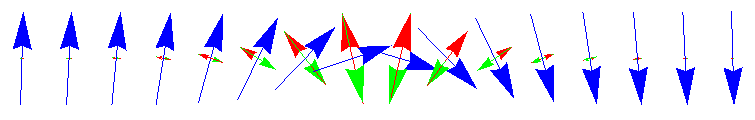
\includegraphics[width=1.0\linewidth]{Figures/NeelJeGTJcAdSTTMS.png}
  \caption{}
  \label{fig:Neel_AdSTT_Heff_JeGTJc}
\end{subfigure}
\begin{subfigure}{\textwidth}
  \centering
  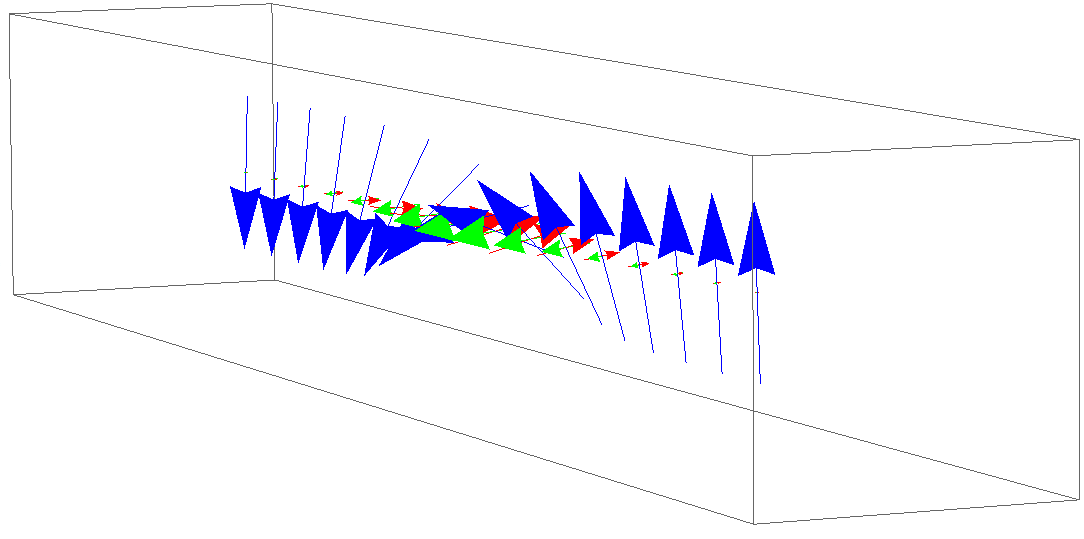
\includegraphics[width=1.0\linewidth]{Figures/NeelJeGTJcNonAdSTTGD.png}
  \caption{}
  \label{fig:Neel_NonAdSTT_GD_JeGTJc}
\end{subfigure}
\caption{The shape of the domain wall different torques acting on it with an applied current $j_e=1.1j_c$. Expectation values are assumed. The blue vectors represent the domain wall magnetization in both figures. In (a) the red vectors represent the adiabatic spin-transfer torque and the green vectors the magnetostatic torque from the effective field. In (b) the red vectors represent the non-adiabatic spin-transfer torque and the green vectors the Gilbert damping torque. The magnitude of the torques are not to scale. The electrons in the applied current move from the domain with spin up to the domain with spin down.}
\label{fig:DW_JeGTJc}
\end{figure}

\subsubsection{External magnetic field}
Instead of applying a current to move domain walls, one can also apply an external magnetic field. Let us now consider the same system as before when we applied the current, but instead we apply a general magnetic field. This causes a change in the energy density, as we now also get a contribution from the Zeeman energy. From the expression of the Zeeman energy in \eqref{eq:zeemanenergy}, one sees that the total energy density of the system becomes
\begin{align}
\nonumber \epsilon&=\epsilon_E+\epsilon_A+\epsilon_Z=A \left(\frac{\partial \theta}{\partial x}\right)^2 + K\sin^2\theta + K_{\perp} \sin^2\theta\sin^2\phi-\mu_0\vec{M}\cdot\vec{H} \\
&= A \left(\frac{\partial \theta}{\partial x}\right)^2 + K\sin^2\theta + K_{\perp} \sin^2\theta\sin^2\phi-\mu_0M_s\left[(H_x\cos\phi+H_y\sin\phi)\sin\theta+ H_z\cos\theta\right].
\end{align}
This gives us
\begin{align}
\frac{\delta \epsilon}{\delta \theta} &= \mu_0M_s\left[H_z\sin\theta - (H_x\cos\phi+H_y\sin\phi)\cos\theta \right], \\
\frac{\delta \epsilon}{\delta \phi} &= K_{\perp}\sin^2\theta\sin2\phi + \mu_0M_s\sin\theta(H_x\sin\phi-H_y\cos\phi).
\end{align}
If we insert these results into \eqref{eq:LLG_current_explicit_spherical} and let $j_e=0$, we get the equations of motion
\begin{align}
\label{eq:xdot_phidot_hfield}
\begin{pmatrix}
\dot{X} \\ \dot{\phi}
\end{pmatrix} = 
\begin{pmatrix}
\frac{\lambda \tilde{\gamma}}{\mu_0M_s} K_{\perp} \sin2\phi  + \tilde{\gamma}\lambda\alpha H_z - \lambda\tilde{\gamma}\left[H_x(\frac{\alpha\cos\phi}{\tan\theta}-\frac{\sin\phi}{\sin\theta}) + H_y(\frac{\alpha\sin\phi}{\tan\theta}-\frac{\cos\phi}{\sin\theta}) \right] \\
-\frac{\alpha\tilde{\gamma}}{\mu_0M_s} K_{\perp}\sin2\phi + \tilde{\gamma} H_z - \tilde{\gamma}\left[H_x(\frac{\cos\phi}{\tan\theta}+\frac{\alpha\sin\phi}{\sin\theta}) + H_y(\frac{\sin\phi}{\tan\theta}-\frac{\alpha\cos\phi}{\sin\theta}) \right]
\end{pmatrix}.
\end{align}
As one can see, if there is an external magnetic field perpendicular to the easy axis ($z$-axis in this example), the equations of motion will depend on $x$ as $\theta = \theta(x,t)$ and we will get a distortion of the domain wall. As discussed earlier, this motion cannot be described by the variables $X$ and $\phi$. We also see that if we set $H_x = H_y = 0$, so that $H_z = H$, the equations become independent of $x$ and we get a motion of the domain wall where the shape is conserved. Doing this, \eqref{eq:xdot_phidot_hfield} gets a similar form as the equations with an applied current in \eqref{eq:xdot_phidot_v2}. By the same argument, there is a critical field strength $H_c$ above which there is no stable solution of $\phi$. This is the field strength $H$ when $\dot{\phi}=0$ and $\sin2\phi=1$, 
\begin{align}
\label{eq:Hcrit}
H_c = \frac{\alpha K_{\perp}}{\mu_0 M_s}.
\end{align}
We can then rewrite the equation to
\begin{align}
\label{eq:xdot_phidot_hz}
\begin{pmatrix}
\dot{X} \\ \dot{\phi}
\end{pmatrix} = 
\begin{pmatrix}
\frac{\lambda}{\alpha T} \sin2\phi  + \frac{\lambda}{T} \alpha \frac{H}{H_c} \\
-\frac{1}{T}\sin2\phi + \frac{1}{T}\frac{H}{H_c}
\end{pmatrix}.
\end{align}
In the case that $\dot{\phi}=0$ we substitute $\sin2\phi$ from the second equation into the first, and find that
\begin{align}
\dot{X}(H\leq H_c) = \frac{\lambda}{T}\left(\frac{1}{\alpha}+\alpha\right) \frac{H}{H_c}.
\end{align}
As the equation for $\dot{\phi}$ is on the exact same form as \eqref{eq:xdot_phidot_v2} with $j_e/j_c \rightarrow H/H_c$, we can use the result that $\langle\sin2\phi\rangle = (H/H_c)- \sqrt{(H/H_c)^2-1}$ when $\dot{\phi} \neq 0$. The translational speed of the domain wall then becomes
\begin{align}
\langle\dot{X}\rangle (H\geq H_c) = \frac{\lambda}{T} \left[\left(\frac{1}{\alpha}+\alpha\right) \frac{H}{H_c} - \frac{1}{\alpha}\sqrt{\left(\frac{H}{H_c}\right)^2-1} \right].
\end{align}
\begin{figure}[h!]
\begin{center}
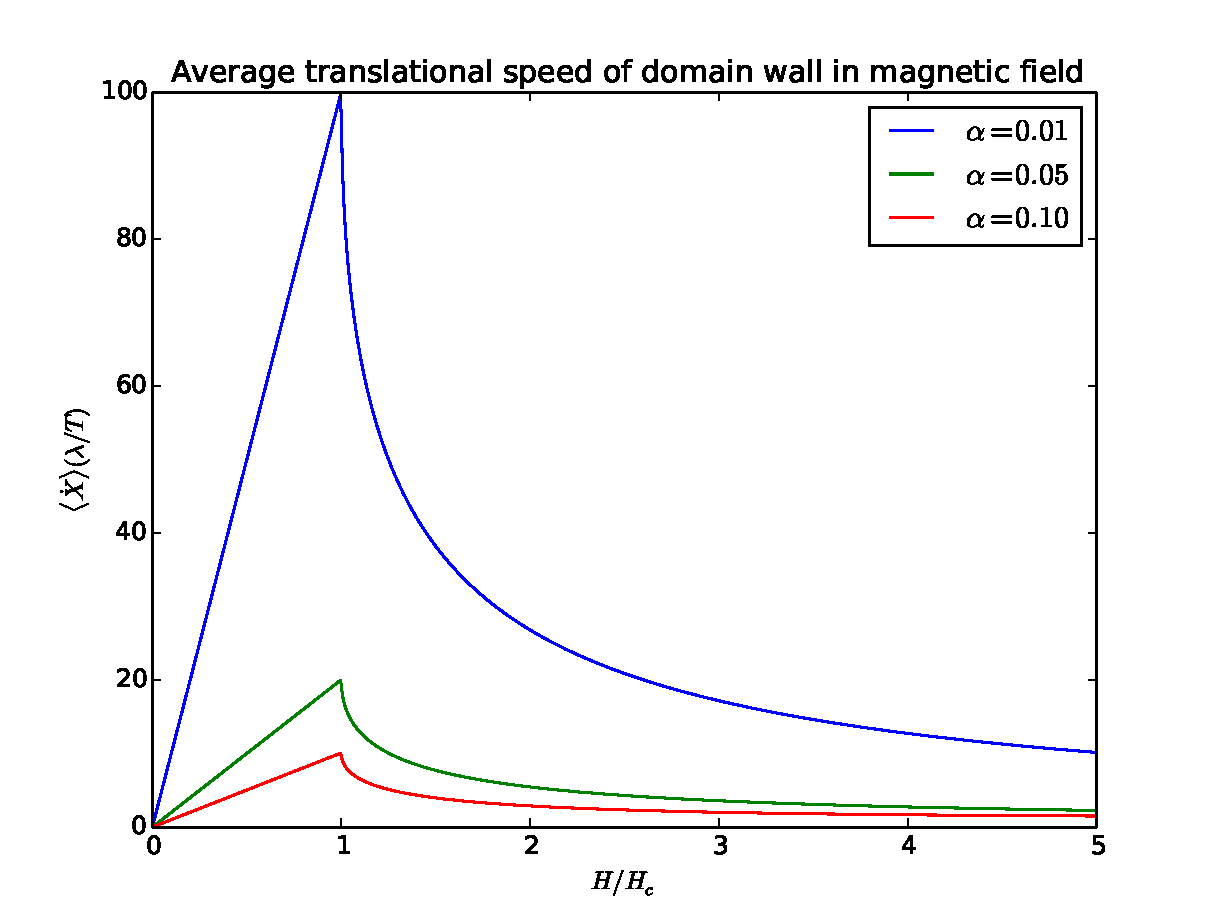
\includegraphics[width=0.8\textwidth]{Figures/criticalField.pdf} 
\caption{The translational speed of the domain wall as a function of applied magnetic field along the easy axis for different damping parameters $\alpha$.}
\label{fig:criticalField} 
\end{center}
\end{figure}
This result is shown in Figure \ref{fig:criticalField}. We see that we also get a Walker breakdown in the case of an applied magnetic field. The rotational speed of the domain wall is entirely equivalent with that of the case with an applied current, as shown in Figure \ref{fig:phidot_afo_current} (with $j_e/j_c \rightarrow H/H_c$). Below the critical field strength the translational speed is proportional to $\alpha^{-1}$, while the critical field strength is proportional to $\alpha$. This means it is possible to achieve high speeds with a relatively weak applied field if the damping parameter $\alpha$ is small. When the damping is small, the magnetization is initially tilted out of the plane, making the component perpendicular to the external field larger. This in turn increases the precession rate of the magnetization. As the damping is proportional to $\alpha$ and $|\frac{\textrm{d} \vec{M}}{\textrm{d} t}|$ the precession rate is allowed to grow significantly before the damping becomes large enough to stop it from increasing further. There is always a decrease in the translational velocity right after the Walker breakdown at $H=H_c$ as the Gilbert damping torque does not have a counterpart like in the motion due to a current, and there is a loss to the rotational motion once there is no longer a stable value for $\phi$. As $H\gg H_c$ the average translational speed becomes proportional to $\alpha$. For small $\alpha$ it is therefore best to apply a field $H$ equal to the critical field strength $H_c$ to obtain the highest translational speed of the domain wall.

One will notice that in dissipationless materials ($\alpha = 0$), the domain wall velocity diverges to $\infty$. This is an unphysical solution, and one must therefore conclude that the assumptions made to get this solution do not hold in this case. The main assumption made was that the domain wall motion could be described by the time dependent coordinates $X$ and $\phi$. It turns out, however, that in a dissipationless material another type of motion becomes available at weak external fields. This motion is known as the breathing mode of the domain wall. The name describes the oscillation of the domain wall width $\lambda$ during the motion of the domain wall, as it expands and shrinks periodically. This type of domain wall propagation was described by Wang et al. \cite{Wang2012}. Their physical picture of the propagation is that the external field causes the domain wall magnetization to precess around the field direction, generating an internal field that is non-uniform in the material. This causes the "breathing" of the domain wall, which in turn emits spin waves from the domain wall center. The emission of these spin waves is what drives the propagation of the domain wall. The spin waves also occur in materials with $\alpha > 0$ and will contribute to the domain wall propagation, but as the dissipation of these become significant for increasing $\alpha$ the contribution to the domain wall propagation decreases. The observant reader will also notice that there is a possible singularity in the current driven domain wall case like in the field driven case, as the final domain wall speed is proportional to $\xi/\alpha$ below the critical current as seen in \eqref{eq:xdot_undercrit}. It is reasonable to assume, however, that if the local magnetization is dissipationless, the magnetization of the conduction electrons will also be dissipationless. The ratio $\xi/\alpha$ can therefore be a finite value, and needs not necessarily diverge.

The reason behind the motion of the domain wall because of a magnetic field parallel to the easy axis is quite easy to understand phenemenologically. As the domains in the magnet are either parallel or anti-parallel to the applied magnetic field, the domain that is parallel will want to grow to minimize the Zeeman energy. This comes at the cost of the anti-parallel domain, and the domain wall moves into the anti-parallel domain as a consequence.

\section{Skyrmions} \label{sec:Skyrmions}
\subsection{Skyrmion profile} \label{sec:SkyrmionProfile}
Skyrmions are stable vortex-like magnetization configurations that appear in materials such as chiral magnets, where the before-mentioned Dzyaloshinskii-Moriya interaction allows the energy of the magnet be lowered by having a slight canting of the neighboring spins. Other interactions may also cause stable skyrmions in a magnet, such as long-ranged magnetic dipolar interactions, frustrated exchange interactions or four-spin exchange interactions. These will typically create skyrmions of a different size than the Dzyaloshinskii-Moriya interaction, which creates skyrmions on a typical length scale of 5-\SI{100}{nm} \cite{Nagaosa2013}. Only skyrmions created by the Dzyaloshinskii-Moriya interaction will be considered here.

To describe the profile of skyrmions, we make an ansatz based on the following: the skyrmion is located in a plane, the out-of-plane magnetization component is azimutally symmetric about the center of the skyrmion, and the in-plane magnetization component is linearly related to the angle in the plane of the skyrmion. Together, this means that the magnetization of the skyrmion can be written as
\begin{align}
\label{eq:SkyrmionMVec}
\vec{M}(\rho, \phi) = M_s
\begin{pmatrix}
\cos\Phi(\phi)\sin\theta(\rho) \\ \sin\Phi(\phi)\sin\theta(\rho) \\ \cos\theta(\rho)
\end{pmatrix}.
\end{align}
Here $\rho$ and $\phi$ denote the in-plane distance from the skyrmion core and the in-plane angle, respectively. The angles $\theta$ and $\Phi$ describe the out-of-plane and in-plane components of the magnetization, with $\theta = \frac{\pi}{2}$ being in-plane and the angle $\Phi$ is related to the in-plane angle of the coordinate system $\phi$ by
\begin{align}
\label{eq:SkyrmionPhi}
\Phi = m\phi + \psi.
\end{align}
Here $m$ is restricted to be an integer due to the symmetry of the problem, and is known as the vorticity of the skyrmion. The absolute value of $m$ tells us how many full rotations the in-plane magnetization makes in the skyrmion plane, while the sign of $m$ tells us if the magnetization rotates with or against the in-plane angle $\phi$. In the special cases $m=1$ and $m=-1$ we get a vortex and an anti-vortex, respectively. The constant phase shift $\psi$ between $\Phi$ and $\phi$ is known as the helicity of the skyrmion. We can then use this ansatz to find an expression for the DMI energy density. Plugging \eqref{eq:SkyrmionMVec} into the bulk form of the DMI energy density in \eqref{eq:BulkDMI} and keeping in mind that
\begin{align}
\frac{\partial \theta}{\partial x} = \cos\phi \frac{\partial\theta}{\partial\rho}, \hspace{5mm}
\frac{\partial \theta}{\partial y} = \sin\phi \frac{\partial\theta}{\partial\rho}, \hspace{5mm}
\frac{\partial \Phi}{\partial x} = -\frac{m}{\rho}\sin\phi, \hspace{5mm}
\frac{\partial \Phi}{\partial y} = \frac{m}{\rho}\cos\phi,
\end{align}
we find that
\begin{align}
\nonumber \epsilon_{DM}^{(\text{bulk})} &= \frac{D}{M_s^2} \vec{M}\cdot(\nabla\times\vec{M}) \\
\nonumber &= D\left(\sin\Phi\cos\phi-\cos\Phi\sin\phi\right)\left[\frac{\partial\theta}{\partial\rho}+\frac{m}{\rho}\sin\theta\cos\theta\right] \\
&= D\sin((m-1)\phi+\psi)\left[\frac{\partial\theta}{\partial\rho}+\frac{m}{\rho}\sin\theta\cos\theta\right].\label{eq:BulkDMIepsilon}
\end{align}
We then choose the degrees of freedom $m$ and $\psi$ that the skyrmion has to minimize the antisymmetric exchange energy. If there is a dependence on $\phi$, the average antisymmetric exchange energy over the plane becomes zero as the function is harmonic. Setting $m=1$ makes this dependence vanish, however, allowing us to have a net negative energy contribution. The choice of $\psi$ is limited to $\pm \frac{\pi}{2}$, with a sign that depends on the sign of $D$ and the profile $\theta(\rho)$. Assuming the expression inside the bracket is negative, the helicity is $\psi = \frac{\pi}{2}$ if $D>0$, and $\psi = -\frac{\pi}{2}$ if $D<0$. We can also perform the same calculation for the interface form of the DMI energy density by plugging our ansatz into \eqref{eq:IntDMI},
\begin{align}
\nonumber \epsilon_{DM}^{(\text{interface})} &= \frac{D}{M_s^2}\left[ M_z (\nabla\cdot\vec{M}) - (\vec{M}\cdot\nabla)M_z\right] \\
\nonumber &= D\left(\sin\Phi\sin\phi+\cos\Phi\cos\phi\right)\left[\frac{\partial\theta}{\partial\rho}+\frac{m}{\rho}\sin\theta\cos\theta\right] \\
&= D\cos((m-1)\phi+\psi)\left[\frac{\partial\theta}{\partial\rho}+\frac{m}{\rho}\sin\theta\cos\theta\right].\label{eq:IntDMIepsilon}
\end{align}
The interface DMI energy density has the same form as the bulk DMI energy density, with the only exception being that it has a cosine instead of a sine. This means that instead of having the stable solutions $\psi = \pm \frac{\pi}{2}$, we now have the stable solutions $\psi=0$ or $\psi=\pi$, depending on the sign of $D$. The in-plane magnetization direction for the different helicities is shown in Figure \ref{fig:m_psi_shapes}. As one can see, for the interface DMI the magnetization will either point away or towards the core of the skyrmion. For the bulk DMI the magnetization will spiral around the core.
\begin{figure}[h!]
\centering
\begin{subfigure}{.49\textwidth}
  \centering
  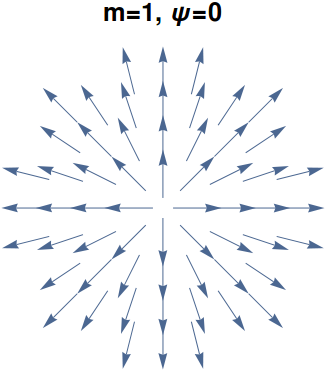
\includegraphics[width=.6\linewidth]{Figures/m1psi0.png}
  \caption{}
  \label{fig:m1psi0}
\end{subfigure}
\begin{subfigure}{.49\textwidth}
  \centering
  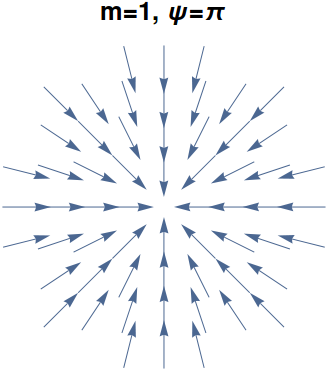
\includegraphics[width=.6\linewidth]{Figures/m1psipi.png}
  \caption{}
  \label{fig:m1psipi}
\end{subfigure}
\begin{subfigure}{.49\textwidth}
  \centering
  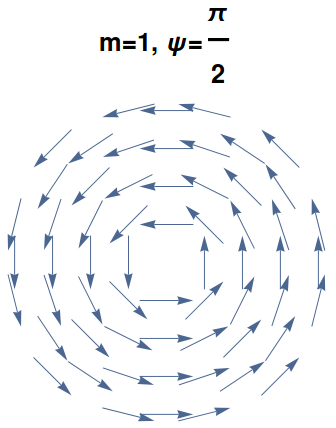
\includegraphics[width=.6\linewidth]{Figures/m1psipi2.png}
  \caption{}
  \label{fig:m1psipi2}
\end{subfigure}
\begin{subfigure}{.49\textwidth}
  \centering
  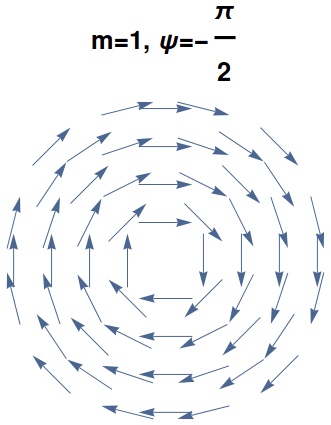
\includegraphics[width=.6\linewidth]{Figures/m1psi-pi2.png}
  \caption{}
  \label{fig:m1psi-pi2}
\end{subfigure}
\caption{The direction of the in-plane magnetization for different helicities $\psi$. }
\label{fig:m_psi_shapes}
\end{figure}
The degrees of freedom of the in-plane magnetization profile have now been determined. To fully describe the profile of the skyrmion all that is left is to find the radial function of the out-of-plane component described by $\theta(\rho)$. This is done by requiring a minimum in the energy, meaning $\frac{\delta E}{\delta\theta} = 0$. As the magnetization is now a function in cylindrical coordinates, we must first find an expression for the symmetric exchange interaction energy density given our ansatz in \eqref{eq:SkyrmionMVec}. Using our previous result in \eqref{eq:exchangeenergyDiv2} and plugging in our ansatz, we find that
\begin{align}
\nonumber\epsilon_E &= \sum_i (\nabla_i\vec{M})\cdot(\nabla_i\vec{M}) \\
\nonumber&= \left(\frac{\partial \vec{M}}{\partial\rho}\right)^2+\frac{1}{\rho^2}\left(\frac{\partial\vec{M}}{\partial\phi}\right)^2+\left(\frac{\partial\vec{M}}{\partial z}\right)^2\\
&= \left(\frac{\partial \theta}{\partial\rho}\right)^2+\frac{\sin^2\theta}{\rho^2}, \label{eq:SymExchCylindrical}
\end{align}
where we have used that $(\frac{\partial\Phi}{\partial\phi})^2=m^2=1$. The total energy can then be written as
\begin{align}
E = \int_{-\infty}^{\infty}\d z \int_0^{2\pi} \d\phi\int_0^{\infty} \d\rho \rho \left(\epsilon_E + \epsilon_{DM} + \epsilon_A\right)
\end{align}
under the assumption that there is no external field and that the demangetization field is incorporated into the anisotropic energy density $\epsilon_A$. As there is no dependence on $z$ or $\phi$, we want to minimize the integral over $\rho$. This means we must require
\begin{align}
\frac{\delta \left[\rho\left(\epsilon_E+\epsilon_{DM}+\epsilon_A\right)\right]}{\delta\theta} = \frac{\partial}{\partial\theta}\left[\rho\left(\epsilon_E+\epsilon_{DM}+\epsilon_A\right)\right] - \frac{\textrm{d}}{\textrm{d}\rho} \frac{\partial}{\partial(\frac{\partial \theta}{\partial\rho})}\left[\rho\left(\epsilon_E+\epsilon_{DM}+\epsilon_A\right)\right] = 0.
\end{align}
We now consider two different examples: a bulk magnet with an easy axis along the $z$-axis, and a thin film with a perpendicular anisotropy and an interface DMI at the surface of the film. For the bulk magnet the anisotropic energy density is given by $\epsilon_A = K\sin^2\theta$ ($K>0$). Combining this with the result we aquired for the bulk DMI and symmetric exchange energy densities in \eqref{eq:BulkDMIepsilon} and \eqref{eq:SymExchCylindrical}, we get the second order differential equation
\begin{align}
\label{eq:ODEthetaBulk}
\frac{\partial^2\theta}{\partial\tilde{\rho}^2} + \frac{1}{\tilde{\rho}}\frac{\partial\theta}{\partial\tilde{\rho}} - \frac{\sin\theta\cos\theta}{\tilde{\rho}^2}+\sin\psi\frac{\sin^2\theta}{\tilde{\rho}}-\frac{AK}{D^2}\sin\theta\cos\theta = 0,
\end{align}
where we have introduced the dimensionless $\tilde{\rho} = \frac{A}{D}\rho$. For the thin film case most of the calculation is exactly the same, with the exception that in $\epsilon_{DM}$ we get $\sin\psi\rightarrow\cos\psi$ and the perpendicular anisotropic energy is given by $K\cos^2\theta$. We therefore pick up a negative sign for the anisotropy term, giving us the differential equation
\begin{align}
\label{eq:ODEthetaFilm}
\frac{\partial^2\theta}{\partial\tilde{\rho}^2} + \frac{1}{\tilde{\rho}}\frac{\partial\theta}{\partial\tilde{\rho}} - \frac{\sin\theta\cos\theta}{\tilde{\rho}^2}+\cos\psi\frac{\sin^2\theta}{\tilde{\rho}}+\frac{AK}{D^2}\sin\theta\cos\theta = 0.
\end{align}
With exception of the trivial solutions $\theta = n\pi$ ($n = 0, 1, 2 \ldots$), \eqref{eq:ODEthetaBulk} and \eqref{eq:ODEthetaFilm} cannot be solved analytically. The trivial solutions are of no interest as the system can reach a lower energy state by having $\frac{\partial\theta}{\partial\rho}\neq 0$ due to the Dzyaloshinskii--Moriya interaction. For the thin film case the trivial solutions are also not stable, as the magnetization will be in the plane of the film far away from the skyrmion core ($\theta=\frac{\pi}{2}$) under the assumption of a hard axis perpendicular to the film. This not a solution of \eqref{eq:ODEthetaFilm}, we therefore see that in the thin-film case it is necessary to have an out-of-plane magnetization component near the skyrmion core. Note that we can also have a thin-film with an easy axis perpendicular to the film, which is called perpendicular magnetic anisotropy. In this case we will get the $\theta(\rho)$ solution of the bulk DMI case, but keep the helicities $\psi = 0, \pi$ of the interface DMI case. This particular skyrmion is often called a hedgehog skyrmion, due to its appearance.

To find the radial profile of the out-of-plane magnetization of the skyrmion one must therefore either solve the equations numerically or use a variational approach to estimate the function $\theta(\rho)$. We solve the equations numerically in MATLAB, imposing the boundary conditions $\theta(0) = 0$ ($\theta(0) = \pi$) and $\theta(\infty) = \pi$ ($\theta(\infty) = 0$) for the bulk case in \eqref{eq:ODEthetaBulk}, and for the interface case in \eqref{eq:ODEthetaFilm} we impose $\theta(0) = 0$ ($\theta(0) = \pi$) and $\theta(\infty) = \pi/2$. For the bulk case we used that the magnetization inside the skyrmion core and the magnetization far away from the core should be parallel to the easy-axis in the $z$-direction, and anti-parallel to each other. For the interface case we imagine a thin film where the magnetization is in the plane far away from the core, and points out of the plane in the core. We have listed two possible boundary conditions for each case that satiesfies this. Which of boundary conditions we use depends on the value of $\psi$, as the solutions acquired numerically only makes sense for one of the boundary conditions. From \eqref{eq:ODEthetaBulk} and \eqref{eq:ODEthetaFilm} one can also see that the solutions for the two different helicities are related to each other by $\theta_{\psi_1}(\rho) = \pi - \theta_{\psi_2}(\rho)$, as the term involving $\psi$ switches sign when the other helicity is chosen, and $\sin(\pi-\theta) = \sin\theta$, $\cos(\pi-\theta) = -\cos\theta$. This means that the solutions for the different values of $\psi$ are simply a mirror image of each other with the mirror being in the skyrmion plane. The numerical solutions for one choice of $\psi$ for both the bulk and interface DMI cases are shown in Figure \ref{fig:ThetaRho}. The initial guesses of the solutions used as an input in the numerics were
\begin{align}
\theta^{\text{(interface)}}(\rho) &= \arctan\tilde{\rho}, \\
\theta^{\text{(bulk)}}(\rho) &= \frac{\pi}{\cosh^2\tilde{\rho}}.
\end{align}
Here we have only considered the profile of the skyrmion in the absence of a magnetic field. One can also have stable skyrmion profiles in a magnetic field, and these profiles will be slightly modified with regards to our solutions without a field. For the effects of an external field and the demagnetization field on the skyrmion profile, one can take a look at the numerical solutions provided by Knoester et al. \cite{Knoester2014}.
\begin{figure}[h!]
\centering
\begin{subfigure}{.49\textwidth}
  \centering
  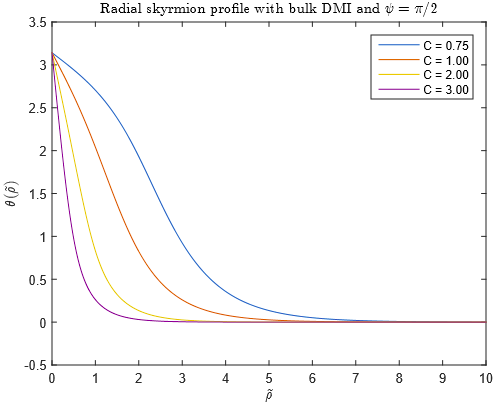
\includegraphics[width=\linewidth]{Figures/ThetaRhoBulk.png}
  \caption{}
  \label{fig:ThetaBulk}
\end{subfigure}
\begin{subfigure}{.49\textwidth}
  \centering
  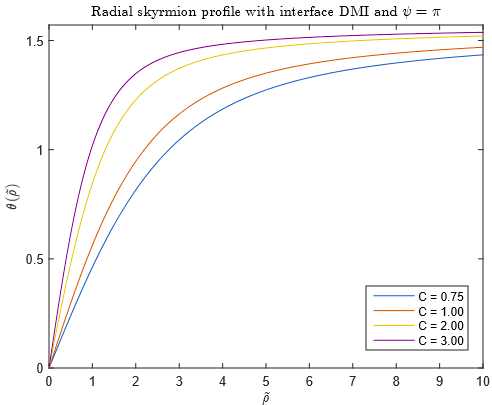
\includegraphics[width=\linewidth]{Figures/ThetaRhoInterface.png}
  \caption{}
  \label{fig:ThetaInt}
\end{subfigure}
\caption{The radial profile of the out-of-plane magnetization component of the skyrmion $\theta(\tilde{\rho})$ for the different forms of the DMI. For the other possible choice of $\psi$ the solution is given by $\pi - \theta(\tilde{\rho})$. $C$ is defined as the variable constant $AK/D^2$ in the differential equation.}
\label{fig:ThetaRho}
\end{figure}

\subsection{Motion of skyrmions} \label{sec:SkyrmionMotion}
To see how skyrmions move under an applied electrical current or an external magnetic field, we use the implicit LLG equation in spherical coordinates, similar to our approach for the domain wall motion when we used the explicit form given by \eqref{eq:LLG_current_explicit_spherical}. The implicit equation is aquired by a similar procedure as the explicit equation was aquired, but now using \eqref{eq:LLG_current} as a starting point. The end result is the following equations:
\begin{align}
\nonumber \begin{pmatrix}
0 \\ \dot{\theta} \\ \sin\theta\dot{\Phi}
\end{pmatrix} =
&\frac{\gamma'}{\mu_0 M_s}
\begin{pmatrix}
0 \\ -\frac{1}{\sin\theta} \frac{\delta \epsilon}{\delta \Phi} \\ \frac{\delta \epsilon}{\delta \theta}
\end{pmatrix} + \alpha
\begin{pmatrix}
0 \\ -\sin\theta\dot{\Phi} \\ \dot{\theta}
\end{pmatrix} + b_J
\begin{pmatrix}
0 \\ (\hat{j}_e\cdot\nabla)\theta \\ \sin\theta(\hat{j}_e\cdot\nabla)\Phi
\end{pmatrix} \\
&+\xi b_J
\begin{pmatrix}
0 \\ \sin\theta(\hat{j}_e\cdot\nabla)\Phi \\ -(\hat{j}_e\cdot\nabla)\theta
\end{pmatrix}.
\label{eq:LLG_current_implicit_spherical}
\end{align}
To describe the motion of a non-deforming skyrmion, we use our ansatz that\\ $\theta = \theta(|\vec{\rho}-\vec{\rho}_0(t)|)$ with both $\vec{\rho}$ and $\vec{\rho}_0(t)$ being in the $xy$-plane and $\vec{\rho}_0(t)$ describing the position of the skyrmion core. For the azimuthal angle $\phi$ defined as the angle between the angle between the $x$-axis and the line intersecting a point in the $xy$-plane and the skyrmion core, we use the ansatz
\begin{align}
\tan\phi = \frac{y-y_0(t)}{x-x_0(t)}.
\end{align}
Note that in a more general approach we would also let the helicity $\psi$ in the in-plane magnetization angle $\Phi$ also be dependent on time, but as we only have two non-trivial equations to solve and already have the two variables $\dot{x}_0$ and $\dot{y}_0$ this is not feasible.

As we removed the dependency on $\phi$ in the energy density by setting $m=1$, we have that $\frac{\delta \epsilon}{\delta \Phi} = 0$. We also used the condition $\frac{\delta\epsilon}{\delta\theta}=0$ to determine $\theta(\rho)$, a condition that still holds in the absence of an external magnetic field. The effective field term in \eqref{eq:LLG_current_implicit_spherical} therefore reduces to an external field under the assumption that the skyrmion is not deformed during its motion.

\subsubsection{Spin-transfer torque}
First we consider the motion of a skyrmion due to the spin-transfer torque from a uniformly applied current in the $x$-direction. As we do not consider the case with an external magnetic field yet, the effective field term vanishes altogether. Defining $r = |\vec{\rho}-\vec{\rho}_0(t)|$, we find the derivatives of $\theta$ and $\phi$ using our ansatz:
\begin{align}
\dot{\theta} &= -\frac{\partial\theta}{\partial r}(\cos\phi\dot{x}_0+\sin\phi\dot{y}_0), \\
\dot{\phi} &= \frac{1}{r}(\sin\phi\dot{x}_0-\cos\phi\dot{y}_0), \\
\frac{\partial \theta}{\partial x} &= \frac{\partial\theta}{\partial r} \cos\phi,\\
\frac{\partial\phi}{\partial x} &= -\frac{\sin\phi}{r}.
\end{align}
Plugging these into \eqref{eq:LLG_current_implicit_spherical} and rearranging the terms gives us the following equations:
\begin{align}
\left(\alpha\frac{\sin\theta}{r}\sin\phi-\frac{\partial\theta}{\partial r}\cos\phi\right)\dot{x}_0 - \left(\alpha\frac{\sin\theta}{r}\cos\phi+\frac{\partial\theta}{\partial r}\sin\phi\right)\dot{y}_0 &= b_J \frac{\partial\theta}{\partial r}\cos\phi - \xi b_J \frac{\sin\theta}{r}\sin\phi, \label{eq:skyrmion_llg_eq1}\\
\left(\alpha\frac{\partial\theta}{\partial r}\cos\phi + \frac{\sin\theta}{r}\sin\phi\right)\dot{x}_0 + \left(\alpha\frac{\partial\theta}{\partial r}\sin\phi - \frac{\sin\theta}{r}\cos\phi\right)\dot{y}_0 &= -b_J\frac{\sin\theta}{r}\sin\phi - \xi b_J \frac{\partial\theta}{\partial r}\cos\phi. \label{eq:skyrmion_llg_eq2}
\end{align}
We then proceed by considering linear combinations of these equations. First we multiply \eqref{eq:skyrmion_llg_eq1} by $\frac{\sin\theta}{r \pi}\sin\phi$ and add it to \eqref{eq:skyrmion_llg_eq2} multiplied by $\frac{1}{\pi}\frac{\partial\theta}{\partial r}\cos\phi$. The resulting equation becomes
\begin{align}
\nonumber &\alpha\left[ (\frac{\partial\theta}{\partial r})^2\frac{\cos^2\phi}{\pi} + \frac{\sin^2\theta}{r^2}\frac{\sin^2\phi}{\pi}\right] \dot{x}_0 - \frac{\sin\theta}{r \pi}\frac{\partial\theta}{\partial r}\dot{y}_0 
+ \alpha \left[(\frac{\partial\theta}{\partial r})^2-\frac{\sin^2\theta}{r^2}\right]\frac{\sin\phi\cos\phi}{\pi}\dot{y}_0 \\
= &-b_J\xi\left[ (\frac{\partial\theta}{\partial r})^2\frac{\cos^2\phi}{\pi} + \frac{\sin^2\theta}{r^2}\frac{\sin^2\phi}{\pi}\right]
\end{align}
We then simplify our problem further and assume that the velocity components $\dot{x}_0$ an $\dot{y}_0$ are independent of position. We can therefore integrate over the skyrmion plane to get rid of the dependency on $\phi$ and $r$. As the term proportional to $\alpha\dot{y}_0$ drops out due to the integration over $\phi$, we are left with
\begin{align}
\alpha I_C \dot{x}_0 - 2\dot{y}_0\int_0^{\infty}\d r \sin\theta\frac{\partial\theta}{\partial r} = -b_J\xi I_C,
\end{align}
where we have defined $I_C$ as the integral
\begin{align}
I_C = \int_0^{\infty} \d r \left[ r(\frac{\partial\theta}{\partial r})^2 + \frac{\sin^2\theta}{r}\right] .
\end{align}
The remaining integral can be performed analytically as
\begin{align}
\int_0^{\infty}\d r \sin\theta \frac{\partial\theta}{\partial r} = \int_{\theta(r =0)}^{\theta(r = \infty)}\d \theta \sin\theta = \cos\theta(r = 0) - \cos\theta (r = \infty).
\end{align}
If we then define $\Gamma$ as
\begin{align}
\label{eq:Gamma}
\Gamma = \frac{I_C}{2[\cos\theta(0)-\cos\theta(\infty)]},
\end{align}
we are left with the equation
\begin{align}
\label{eq:skyrmion_xy_eq1}
\alpha\Gamma \dot{x}_0 - \dot{y}_0 = -b_J\xi\Gamma.
\end{align}
We need another equation for $\dot{x}_0$ and $\dot{y}_0$ to find their solutions. To do that we make a different linear combination of \eqref{eq:skyrmion_llg_eq1} and \eqref{eq:skyrmion_llg_eq2}, a linear combination that has to be independent of the first one. This time we multiply \eqref{eq:skyrmion_llg_eq1} by $\frac{\sin\theta}{r \pi}\cos\phi$ and subtract it from \eqref{eq:skyrmion_llg_eq2} multiplied by $\frac{1}{\pi}\frac{\partial\theta}{\partial r}\sin\phi$. The equation we get then is
\begin{align}
\nonumber &\alpha\left[ (\frac{\partial\theta}{\partial r})^2\frac{\sin^2\phi}{\pi} + \frac{\sin^2\theta}{r^2}\frac{\cos^2\phi}{\pi}\right] \dot{y}_0 + \frac{\sin\theta}{r \pi}\frac{\partial\theta}{\partial r}\dot{x}_0 
+ \alpha \left[(\frac{\partial\theta}{\partial r})^2-\frac{\sin^2\theta}{r^2}\right]\frac{\sin\phi\cos\phi}{\pi}\dot{x}_0 \\
= &-b_J\xi\left[ (\frac{\partial\theta}{\partial r})^2 - \frac{\sin^2\theta}{r^2}\right]\frac{\sin\phi\cos\phi}{\pi} - b_J\frac{\sin\theta}{\pi}\frac{\partial\theta}{\partial r}.
\end{align}
Integrating this equation over the skyrmion plane and making the same definitions as before, we finally end up with the equation
\begin{align}
\label{eq:skyrmion_xy_eq2}
\alpha\Gamma\dot{y}_0 + \dot{x}_0 = -b_J.
\end{align}
Solving \eqref{eq:skyrmion_xy_eq1} and \eqref{eq:skyrmion_xy_eq2} for $\dot{x}_0$ and $\dot{y}_0$ we end up with the final expressions for the velocity components of the skyrmion:
\begin{align}
\dot{x}_0 &= -\frac{1+\Gamma^2\alpha\xi}{1+\Gamma^2\alpha^2}b_J, \label{eq:skyrmion_xdot} \\
\dot{y}_0 &= \frac{\Gamma(\xi-\alpha)}{1+\Gamma^2\alpha^2}b_J. \label{eq:skyrmion_ydot}
\end{align}
For the thin film case we have $\theta(0) = 0$ and $\theta(\infty)=\pi/2$, and as the integrand in $I_C$ then becomes proportional to $\rho^{-1}$ as $\rho$ becomes large, the integral and therefore $\Gamma$ diverges. The thin film form of the skyrmion therefore has a velocity that is approximately
\begin{align}
\vec{v} \approx -\frac{\xi}{\alpha}b_J\hat{x}.
\end{align}
This result is equivalent to the result for the motion of the 1D domain wall when an electrical current below the critical current is applied.\\
\begin{table}[h!]
	\centering
		\caption{Values of the integral $I_C$ for different values of $C$, using the bulk solution of $\theta(\rho)$.} 
	\begin{tabular}{l l} \hline
	$C$ & $I_C$\\ \hline
	0.75  & 6.5118\\
 	1.00  & 5.1355\\
 	2.00  & 5.3793 \\ 
 	3.00  & 5.6452 \\ \hline
	\end{tabular}
	\label{tab:C_I}
\end{table}

For the bulk case we have $\theta(0) = \pi$ and $\theta(\infty) = 0$. In this case the integral $I_C$ converges to a value that has to be found numerically. A few example values of $I_C$ are shown in Table \ref{tab:C_I} for different values of $C = AK/D^2$. Using that $\Gamma = -I_C/4$ the resulting velocity becomes
\begin{align}
\vec{v} = -\frac{16+I_C^2\alpha\xi}{16+I_C^2\alpha^2}b_J\hat{x} + \frac{4(\alpha-\xi)I_C}{16+I_C^2\alpha^2}b_J\hat{y}.
\label{eq:SkyrmionV}
\end{align}
As we can see we also have a velocity component in the $y$-direction when $\xi\neq\alpha$. This component perpendicular to the direction of the current originates from the skyrmion Hall effect \cite{Nagaosa2013}\cite{Zang2011}. The skyrmion Hall effect can be understood by the emergent electromagnetic field that arises due to the non-trivial topology of the skyrmion. The skyrmion profile creates an effective magnetic flux \cite{Nagaosa2012}, given by
\begin{align}
\vec{b}_e = \left[\frac{\hbar}{2 e} \hat{M} \cdot \left( \frac{\partial \hat{M}}{\partial x} \times \frac{\partial \hat{M}}{\partial y}\right)\right]\hat{z}.
\end{align}
The total magnetic flux of the skyrmion can be written as a constant times the skyrmion number, defined by \cite{Heinze2011}
\begin{align}
N_{\textrm{sk}} = \frac{1}{4\pi}\int \hat{M}\cdot\left(\frac{\partial \hat{M}}{\partial x} \times \frac{\partial \hat{M}}{\partial y}\right) \d x \d y.
\end{align}
The skyrmion number is only non-zero for non-trivial topological magnetization structures. For the bulk form of the skyrmion profile it can be shown that the skyrmion number is $N_{\textrm{sk}} = 1$ \cite{Nagaosa2013}. Since the skyrmion carries with it a magnetic field, there will also be an emergent electric field $\vec{e}_e$ \cite{Schulz2012} that will balance out the Lorentz force 
\begin{align}
\label{eq:LorentzForce}
\vec{F}_{\textrm{Lorentz}} = q\left[\vec{e}_e + \vec{v}\times\vec{b}_e\right],
\end{align}
meaning the resulting emergent electric field becomes
\begin{align}
\vec{e}_e = -\vec{v}\times\vec{b}_e.
\end{align}
This emergent electric field will then generate a current, and as the field lies in the skyrmion plane and is perpendicular to the direction of the external applied current it accounts for the velocity component we get in the $y$-direction.

\subsubsection{External magnetic field}
If we instead turn off the electrical current and apply an external magnetic field in the $z$-direction, we will now get a non-zero contribution from $\frac{\delta\epsilon}{\delta\theta}$ due to the Zeeman energy. The Zeeman energy density is given by $\epsilon_Z = -\mu_0M_sH\cos\theta$. This leads to the equations of motion in a magnetic field:
\begin{align}
\begin{pmatrix}
\dot{\theta} \\ \sin\theta\dot{\Phi}
\end{pmatrix} =
\begin{pmatrix}
-\alpha \sin\theta\dot{\Phi} \\ \gamma' H\sin\theta + \alpha\dot{\theta}
\end{pmatrix}.
\label{eq:LLG_skyrmion_Hz}
\end{align}
For non-zero $\alpha$ this will lead to a deformation of the skyrmion. Unlike the case with an applied current, $\dot{\theta}$ does not represent a motion of the skyrmion core. The ansatz $\theta = \theta(|\vec{\rho}-\vec{\rho}_0(t)|)$ does not hold anymore. An external magnetic field perpendicular to the skyrmion plane cannot move the skyrmion core, as there is no other location that is more energetically favorable. Instead, $\dot{\theta}$ represents a change in the radial profile of the skyrmion, as the initial profile no longer minimizes the energy when an external field is applied. If $(\gamma'\alpha H)^{-1}$ is large compared to the time-scale on which the system changes, however, this deformation is negligible. The effect of the magnetic field in the $z$-direction is therefore a rotation of the in-plane magnetization of the skyrmion with a precession rate $\dot{\Phi} \approx \gamma'H$. If the applied magnetic field is of a strength so that the deformation is no longer negligible, the skyrmion profile will change towards an equilibrium profile in an external magnetic field (the Zeeman energy is taken into account when determining the $\theta (\rho)$ profile) if the field is applied adiabatically. This means that if one applies an alternating magnetic field perpendicular to the skyrmion plane, one can excite a breathing mode in the skyrmion like in the domain wall case, where the skyrmion core expands and shrinks periodically with the magnetic field \cite{Mochizuki2012}.

\subsection{The Thiele equation}
Magnetization patterns that do not deform during their motion, like the motion of the skyrmion due to a spin-polarized current as shown earlier, can be described by an equation known as the Thiele equation. In \cite{Thiele1973} Thiele recognized that if the magnetization can be written as $\vec{M}(\vec{r}-\vec{R}(t))$, meaning the magnetization pattern moves uniformly, the time derivative can be written as
\begin{align}
\label{eq:ThieleRelation}
\frac{\textrm{d} \vec{M}}{\textrm{d} t} = \frac{\partial \vec{R}}{\partial t}\frac{\partial \vec{M}}{\partial \vec{R}} = \frac{\partial \vec{R}}{\partial t} (-\frac{\partial \vec{M}}{\partial \vec{r}}) = -(\vec{v}\cdot\nabla)\vec{M},
\end{align}
with $\vec{v}$ being the velocity of the magnetization pattern. Here we have used that since the magnetization exclusively depends on the difference between $\vec{r}$ and $\vec{R}(t)$, a small spatial change in $\vec{R}(t)$ can be replaced by a small spatial change in $\vec{r}$ in the opposite direction. This result can then be substituted into the implicit LLG equation in \eqref{eq:LLG_current} to simplify it. 
Another simplification one can make is setting the effective field $\vec{H}_{\text{eff}}$ equal to an external magnetic field $\vec{H}$. This is easily verified as one finds that the skyrmion minimizes the energy from internal effects, meaning $\frac{\delta\epsilon}{\delta\theta}$ and $\frac{\delta\epsilon}{\delta\phi}$ are zero in the absence of an external magnetic field. Together, this means that the LLG equation can be written as
\begin{align}
\gamma'\vec{M}\times\vec{H} - ((\vec{v}+b_J\hat{j}_e)\cdot\nabla)\vec{M} + \frac{1}{M_s}\vec{M}\times((\alpha\vec{v}+\xi b_J\hat{j}_e)\cdot\nabla)\vec{M} = 0.
\end{align}
After a considerable amount of manipulation and rewriting of the equation above, one finally ends up with the Thiele equation:
\begin{align}
\label{eq:Thiele}
\vec{F} + \vec{G}\times(\vec{v}+b_J\hat{j}_e) + \bar{D}(\alpha\vec{v}+\xi b_J\hat{j}_e) = 0.
\end{align}
$\vec{F}$ is the force vector acting on the magnetization pattern, $\vec{G}$ is the gyrovector, and $\bar{D}$ is the dissipation tensor. These have the following definitions:
\begin{align}
\vec{F} &= -\mu_0 \int\d A \left[(\nabla\theta)\frac{\partial}{\partial \theta} + (\nabla\phi)\frac{\partial}{\partial \phi}\right] (\vec{H}\cdot\vec{M}),\label{eq:ThieleForce} \\
\vec{G} &= \frac{2\pi M_s\mu_0}{\gamma'}\left[\cos\theta\right]_{\theta(\rho = 0)}^{\theta(\rho=\infty)} \hat{z} = G_0 \hat{z}, \label{eq:ThieleGyro} \\
\bar{D} &= -\frac{\pi M_s\mu_0}{\gamma'}\int_0^{\infty}\d \rho \left(\rho \left(\frac{\partial \theta}{\partial \rho}\right)^2+\frac{\sin^2\theta}{\rho}\right)(\hat{x}\otimes\hat{x}+\hat{y}\otimes\hat{y}). \label{eq:ThieleDissipation}
\end{align}
A detailed derivation of how to obtain the Thiele equation from the LLG equation using Thiele's relation in \eqref{eq:ThieleRelation} is provided by Kr\"{u}ger in \cite{krugerDissertation}. If one solves the Thiele equation for our example of skyrmion motion due to a spin-polarized current, the end result becomes the same as the one we got by solving the LLG equation directly. This solution will not be shown here, but a simplification of Kr\"{u}ger's solution to our case without finite size effects of the film reduces to the result in \eqref{eq:SkyrmionV}.

The advantage of using the Thiele equation over the LLG equation is that once the profile of the skyrmion is known, the Thiele equation becomes an implicit vector equation for the velocity. The LLG equation, however, is a set of coupled equations in the velocity components. For cases where the skyrmion profile does not change during its motion, it is therefore easier to find the velocity of the skyrmion by using the Thiele equation than the LLG equation, especially as the complexity of the problem increases (for example when including finite film size effects as discussed by Kr\"{u}ger).

\subsection{Research on skyrmions}

\section{Conclusion}
In this thesis we have derived the extended Landau--Lifshitz--Gilbert equation that describes the time evolution of a magnetization structure. This has then been applied to describe the dynamics of different magnetic solitons. These magnetic solitons include magnetic domain walls, as described in chapter \ref{sec:DW}, and magnetic skyrmions, as described in chapter \ref{sec:SkyrmionProfile}. The structure of these magnetic solitons were derived from the micromagnetic energy terms in chapter \ref{sec:MicromagneticEnergy}. For the motion of magnetic domain walls it was discovered in chapter \ref{sec:DWDynamics} that there was a linear relation between the translational speed of the domain wall and the strength of the applied current or magnetic field up to a critical value, after which a Walker breakdown occured. In chapter \ref{sec:SkyrmionMotion} we found that for a weak current the translational speed of a magnetic skyrmion was linearly related to the strength of the applied current. In the case of different damping between the local and itinerant electrons it was also discovered that we get a velocity component perpendicular to the direction of the applied current due to the skyrmion Hall effect.

This thesis exclusively focused on the effects of an electric current or a magnetic field on magnetic solitons. In the future, it may also be of interest to study the effects that an applied electric field may have on the skyrmion, as it can couple to the magnetization via spin-orbit coupling. This can lead to different equilibrium and dynamical properties of the magnetic skyrmion.

\bibliography{main}
\bibliographystyle{unsrt}


\end{document}